\documentclass[30pt, blockverticalspace=1cm]{tikzposter}
\geometry{paperwidth=1978mm,paperheight=1183mm}
\makeatletter
\setlength{\TP@visibletextwidth}{\textwidth-2\TP@innermargin}
\setlength{\TP@visibletextheight}{\textheight-2\TP@innermargin}
\makeatother
%\documentclass[]{beamer}



\title{\parbox{\linewidth}{\centering Rotating Stratified Turbulence
}}
\author{Dante Buhl, Pascale Garaud, Hongyun Wang}
\date{April 29, 2025}
\institute{University of California Santa Cruz, Department of Applied
Mathematics}
\usetheme{Default}
\usecolorstyle{Default}
\usecolorpalette{Default}

%% PACKAGES %%
\usepackage[utf8]{inputenc}
\usepackage{amsmath, amssymb, amsthm}
\usepackage{mathtools}
\usepackage[shortlabels]{enumitem}
\usepackage{tikz}
\usepackage[dvipsnames]{xcolor}
\usepackage[backend=bibtex,style=numeric,sorting=none]{biblatex}
\usepackage{subfig}
\usepackage{verbatim}
\usepackage{enumerate}
\usepackage{graphicx}
\usepackage{bm}

%for positioning nodes
\usetikzlibrary{positioning}
\usepackage[none]{hyphenat}


\begin{document}


\newcommand{\red}{\color{red}}
\newcommand{\wrms}{w_{\text{rms}}}
\newcommand{\bs}[1]{\boldsymbol{#1}}
\newcommand{\tb}[1]{\textbf{#1}}
\newcommand{\bmp}[1]{\begin{minipage}{#1\linewidth}}
\newcommand{\emp}{\end{minipage}}
\newcommand{\R}{\mathbb{R}}
\newcommand{\C}{\mathbb{C}}
\newcommand{\N}{\mathcal{N}}
\newcommand{\K}{\bs{\mathrm{K}}}
\newcommand{\m}{\bs{\mu}_*}
\newcommand{\s}{\bs{\Sigma}_*}
\newcommand{\dt}{\Delta t}
\newcommand{\dx}{\Delta x}
\newcommand{\tr}[1]{\text{Tr}(#1)}
\newcommand{\Tr}[1]{\text{Tr}(#1)}
\newcommand{\Div}{\nabla \cdot}
\renewcommand{\div}{\nabla \cdot}
\newcommand{\Curl}{\nabla \times}
\newcommand{\grad}{\nabla}
\newcommand{\pt}{\partial t}
\newcommand{\pz}{\partial z}
\newcommand{\uvec}{\bs{u}}
\newcommand{\F}{\bs{F}}
\newcommand{\T}{\tilde{T}}
\newcommand{\ez}{\bs{e}_z}
\newcommand{\ex}{\bs{e}_x}
\newcommand{\ey}{\bs{e}_y}
\newcommand{\eo}{\bs{e}_{\bs{\Omega}}}
\newcommand{\ppt}[1]{\frac{\partial #1}{\partial t}}
\newcommand{\DDt}[1]{\frac{D #1}{D t}}
\newcommand{\dd}[2]{\frac{d #1}{d #2}}
\newcommand{\pp}[2]{\frac{\partial #1}{\partial #2}}
\newcommand{\ddz}[1]{\frac{d #1}{d z}}
\newcommand{\ppx}[1]{\frac{\partial #1}{\partial x}}
\newcommand{\ppy}[1]{\frac{\partial #1}{\partial y}}


%% images in corners %%
% need to add UCSC logo
\node [below right=-1cm and 5cm] at (bottomleft |- topright)
{
\includegraphics[width=21cm]{ucsc_logo_2.png}};
\node [below left=-.5cm and 7cm] at (topright) {\includegraphics[width=15cm]{images/NSF-logo.png}};

%% TITLE AND LOGOS %%
\maketitle

\begin{columns}


%%%%%%%%%%%%%%%%%%%%%%%%%%%%%%%%%%%%%%%%%%%%%%%%%%%%%%%%
\column{0.33}
%%%%%%%%%%%%%%%%%%%%%%%%%%%%%%%%%%%%%%%%%%%%%%%%%%%%%%%%


\block{Abstract}
{
Recent interest in the dynamics of stratified turbulence has led to the
development of new models for quantifying vertical transport of momentum and
buoyancy (Chini {\em et al} 2022, Shah {\em et al} 2024). These models are still
incomplete as they do not yet include all of the relevant dynamics often present
in real physical settings such as rotation and magnetic fields. Here we expand
on prior work by adding rotation. We conduct 3D direct numerical simulations of
rotating, stochastically forced, strongly stratified turbulence ($Fr \ll  1$), and vary the Rossby number. We find that rotation gradually suppresses small-scale 3D motions and therefore inhibits vertical transport as Ro decreases towards Fr. The effect is particularly pronounced within the cores of emergent cyclonic vortices. For sufficiently strong rotation, vertical motions are entirely suppressed.
}


\block{Motivation}
{ 
    % TAKE FROM DFD PRESENTATION
\bmp{.47}
    
    Nonrotating stratified turbulence is characterized by strongly
    anisotropic pancake structures within the flow. 

    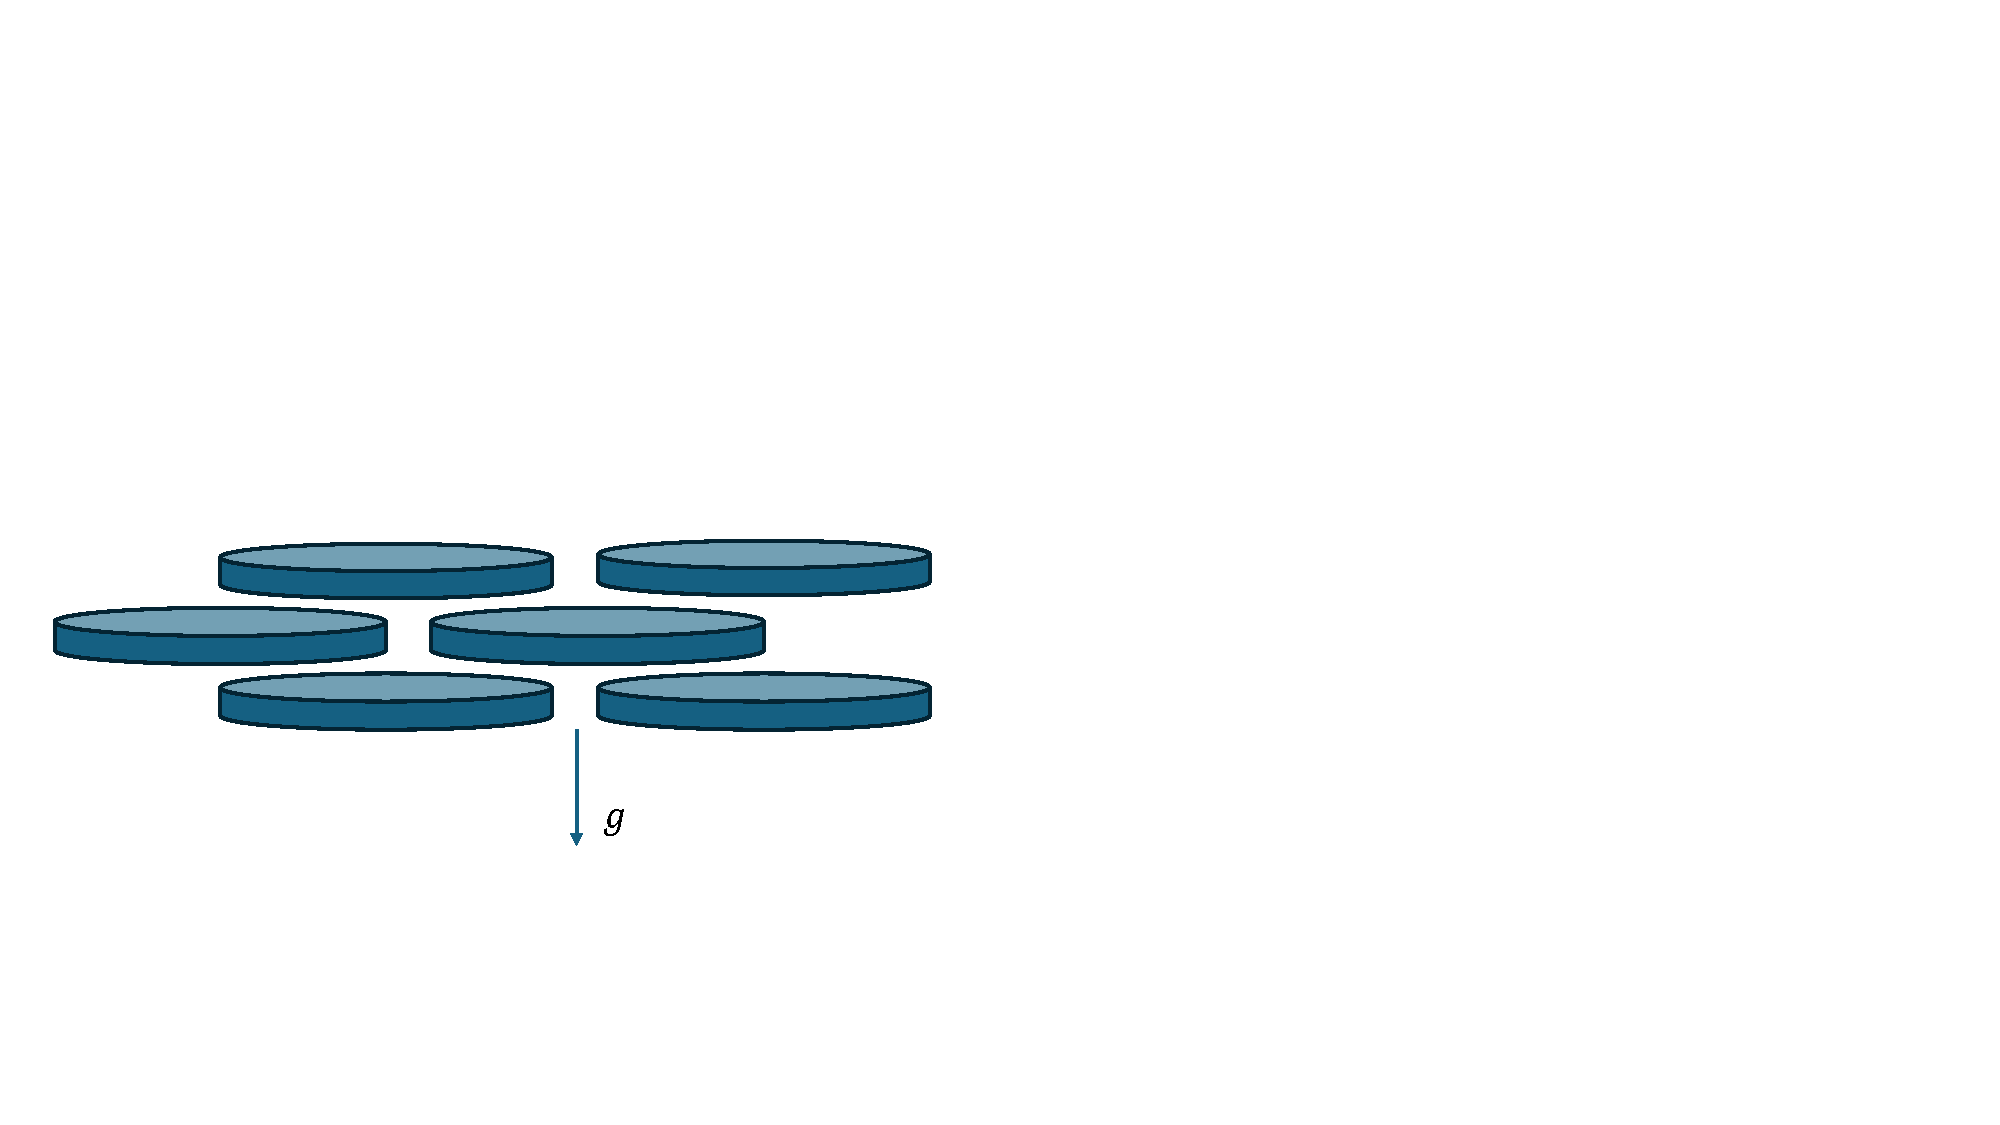
\includegraphics[width=.9\linewidth]{images/pancakes.pdf}
     %end small
\emp
\hfill
\bmp{.47}
    
    Rotation promotes barotropic structures which are invariant along the axis
    of rotation.

    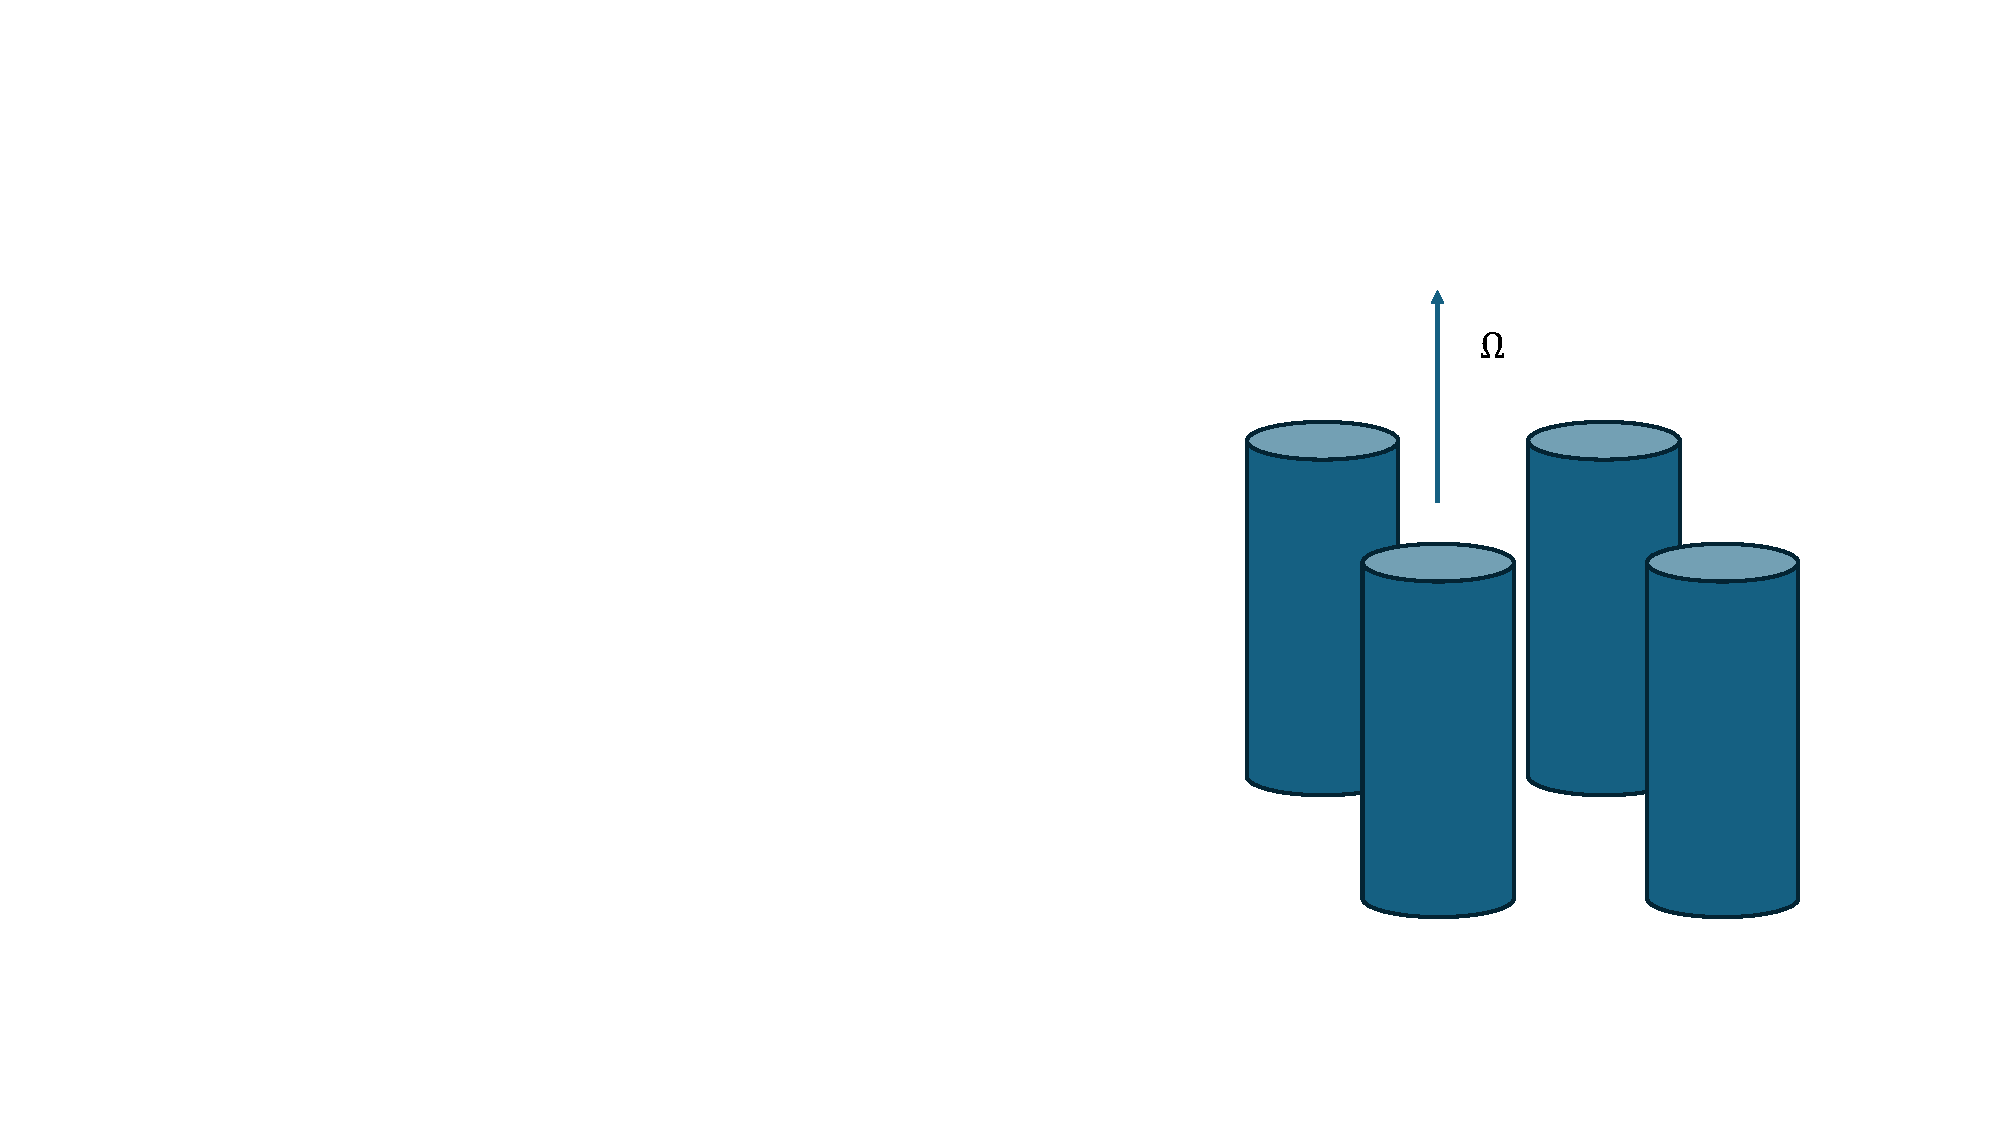
\includegraphics[width=.9\linewidth]{images/cylinders.pdf}
     %end small
\emp
}


\block{The Equations}
{
\centering
\bmp{.35}
We consider a triply periodic domain stably stratified by a mean temperature
profile $\bar{T}$ in the vertical direciton. 

\begin{gather*}
    \DDt{\uvec} + \frac{1}{Ro}\ez\times\uvec = -\grad p + \F +
    \frac{1}{Fr^2}\tilde{T} \ez 
    + \frac{1}{Re} \grad^2 \uvec\end{gather*}
\begin{gather*}
    \div{\uvec} = 0, \quad 
    T = \bar{T}(z) + \tilde{T}, \quad \DDt{\tilde{T}} + w = \frac{1}{Pe} \grad^2\tilde{T}
\end{gather*}
\begin{gather*}
     Re = \frac{UL}{\nu},\quad  Pe = \frac{UL}{\kappa_T},\quad Fr =
    \frac{U}{NL},\quad  Ro =
    \frac{U}{2\Omega L}
\end{gather*}
\emp
\hspace{10pt}
\bmp{.6}
\centering
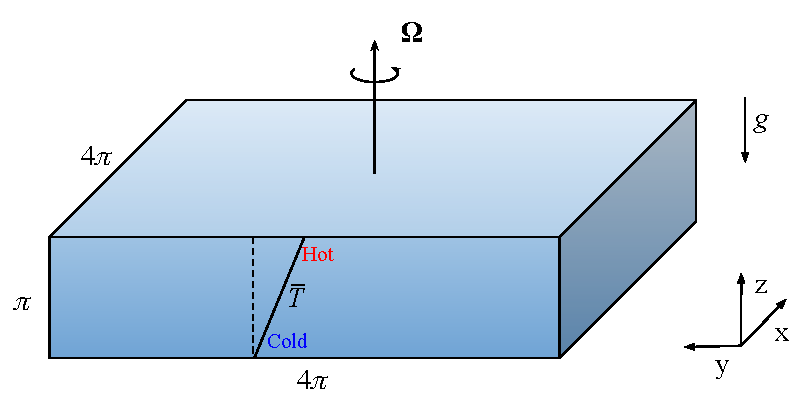
\includegraphics[width=.9\linewidth]{images/schematic.pdf}
\emp
}
\block{Stochastic Forcing}{

    \bmp{.45}
        We choose the forcing to be purely horizontal and divergence-free stochastic
        process:
        \[
            \bs{F} = F_x\ex + F_y\ey, \quad \grad \cdot \bs{F} = 0
        \]
        The forcing is applied in spectral space and satisfies $\bs{k} \cdot \hat{\bs{F}} = 0$:
        \begin{gather*}
            \hat{F}_x = \frac{k_y}{|\bs{k}_h|}G(\bs{k}_h,t), \quad \hat{F}_y = \frac{-k_x}{|\bs{k}_h|}G(\bs{k}_h,t)\\
        \end{gather*}
        where $G(\bs{k}_h,t)$ is a Gaussian process of amplitude 1 and correlation
        timescale 1, and $|\bs{k}_h| \le \sqrt{2}$. The Gaussian process
        timeseries are
        autoregressively generated in spectral space using a pseudo-inverse
        algorithm. The Gaussian kernel is generated using the exponential
        squared kernel function
        \begin{gather*}
            K(t, t') = \exp\left(\frac{-(t - t')^2}{2\tau^2}\right)
        \end{gather*}
        in order to improve smoothness and differentiability of the forcing in
        time. The image on the right depicts an example of the forcing in time
        for a single wavenumber taken from one of the non-rotating simulations. 

        \begin{flushright}
        c.f. Waite and Bartello (2004)\end{flushright}
    \emp
    \bmp{.55}
        \centering
        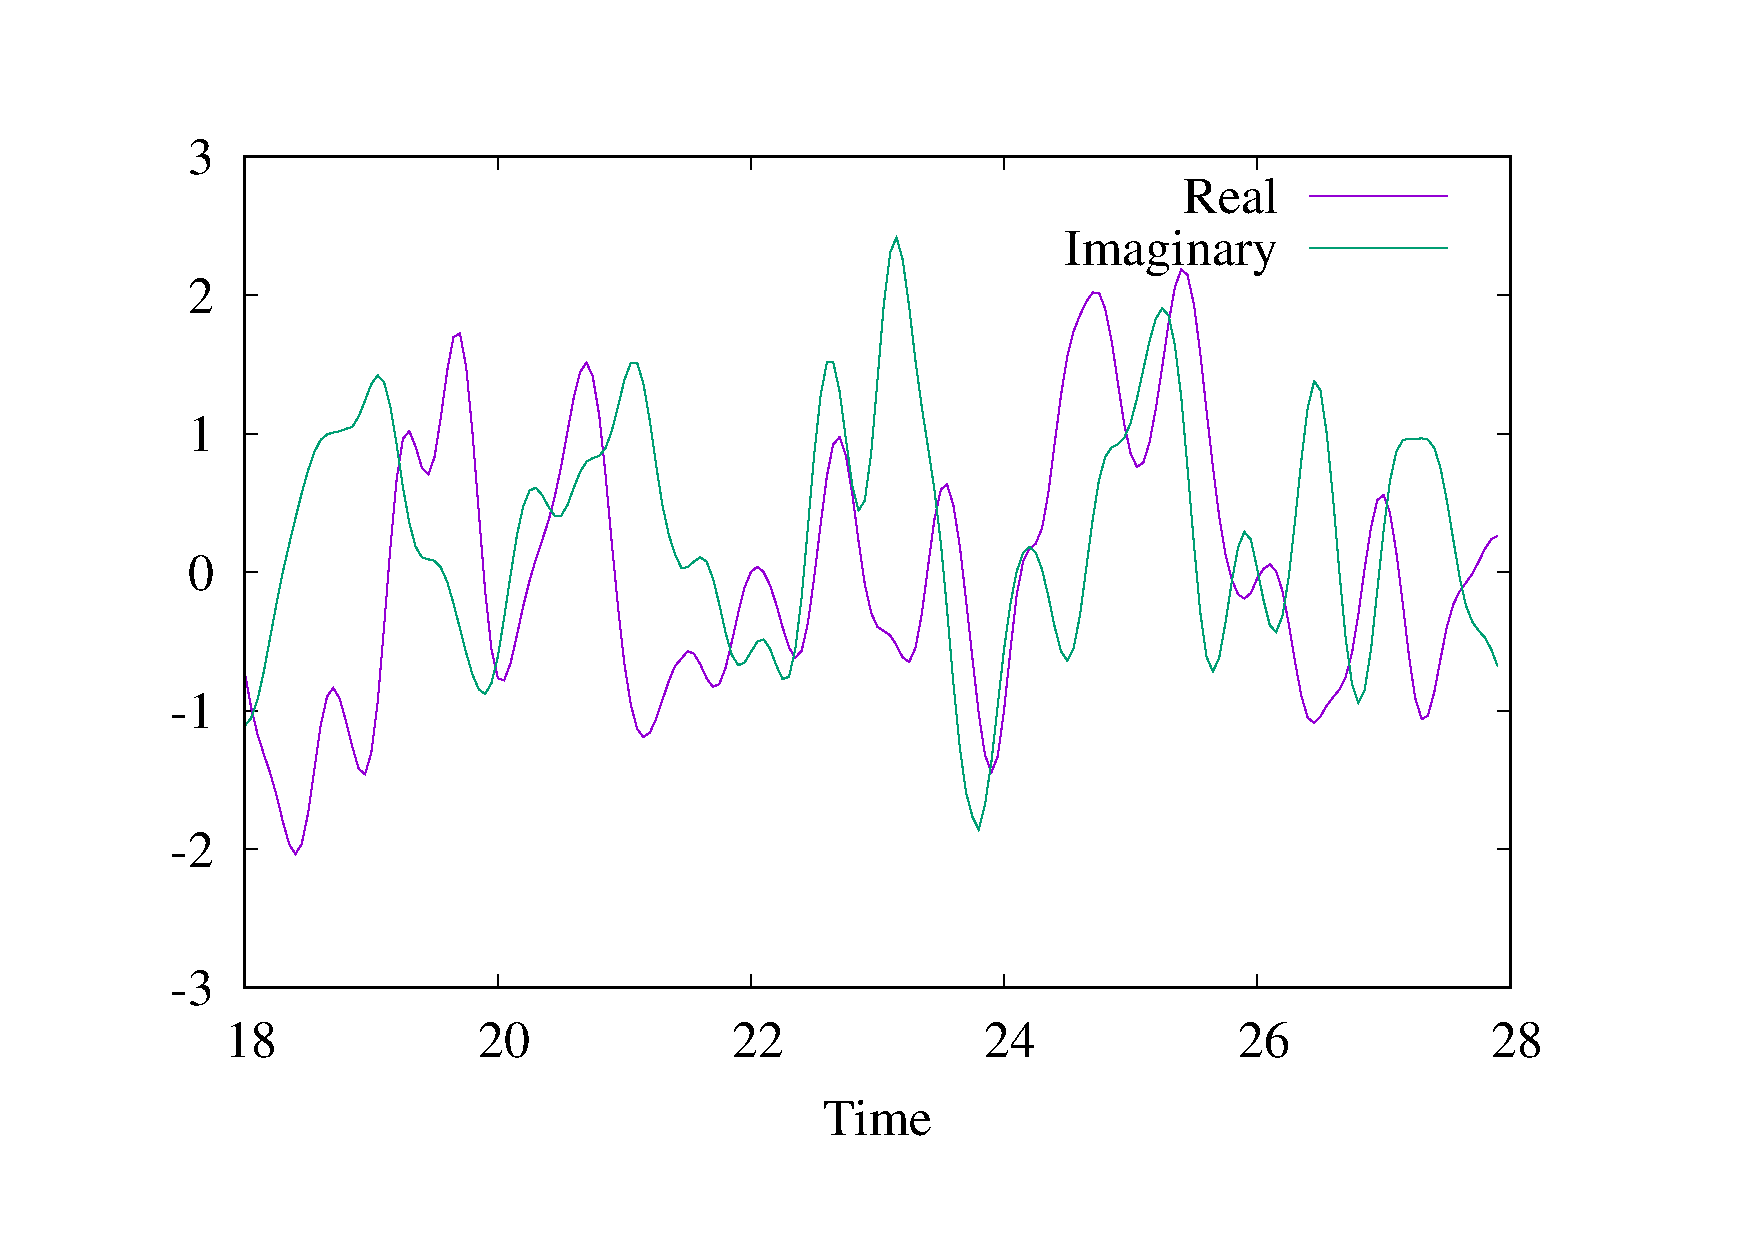
\includegraphics[width=.95\linewidth]{images/forcing_example.pdf}
    \emp
}

%%%%%%%%%%%%%%%%%%%%%%%%%%%%%%%%%%%%%%%%%%%%%%%%%%%%%%%%
\column{0.33}
%%%%%%%%%%%%%%%%%%%%%%%%%%%%%%%%%%%%%%%%%%%%%%%%%%%%%%%%


\block{Simulation Visualization}{
    % start showing data and results. Things to include in this block should be
    % quantitative datas, rms scaling laws with rossby and the such

    Two series of simulations have been conducted with $Re = 600, Pe = 60$
    at two different
    Froude numbers (moderately stratified case $Fr = 0.18$, strongly stratified
    case $Fr = 0.1$). The Rossby number varies in $[0.1, 2]$. The figures below show
    results for $Fr = 0.18$, and increasing rotation rate from left to right. 
    The top row shows volume renderings of the vertical
    component of vorticity. The middle row shows the temperature dissipation.
    The bottom row shows kinetic energy spectra for the horizontal and vertical
    flows. The vorticity renderings illustrates the
    formation of cyclones and anticyclones which exhibit increasing vertical
    invariance as the rotation rate increases. 
    Associated with the emergence of vertically cohearent vortices, we also
    note the appearance of an inverse energy cascade characterized by a
    $\bs{k}_h^{-3}$ spectrum for the horizontal flow. Finally, we see that the
    thermal dissipation becomes negligible inside the cyclones. 

    \begin{center}

    % this may be the appropriate section to include the QR code. 
    \bmp{.09}
        
        \centering
        {\Large $\omega_z$}
    \emp
    \bmp{.3}
        \centering
        {\Large $Ro = 2$}
        \vspace{10pt}

        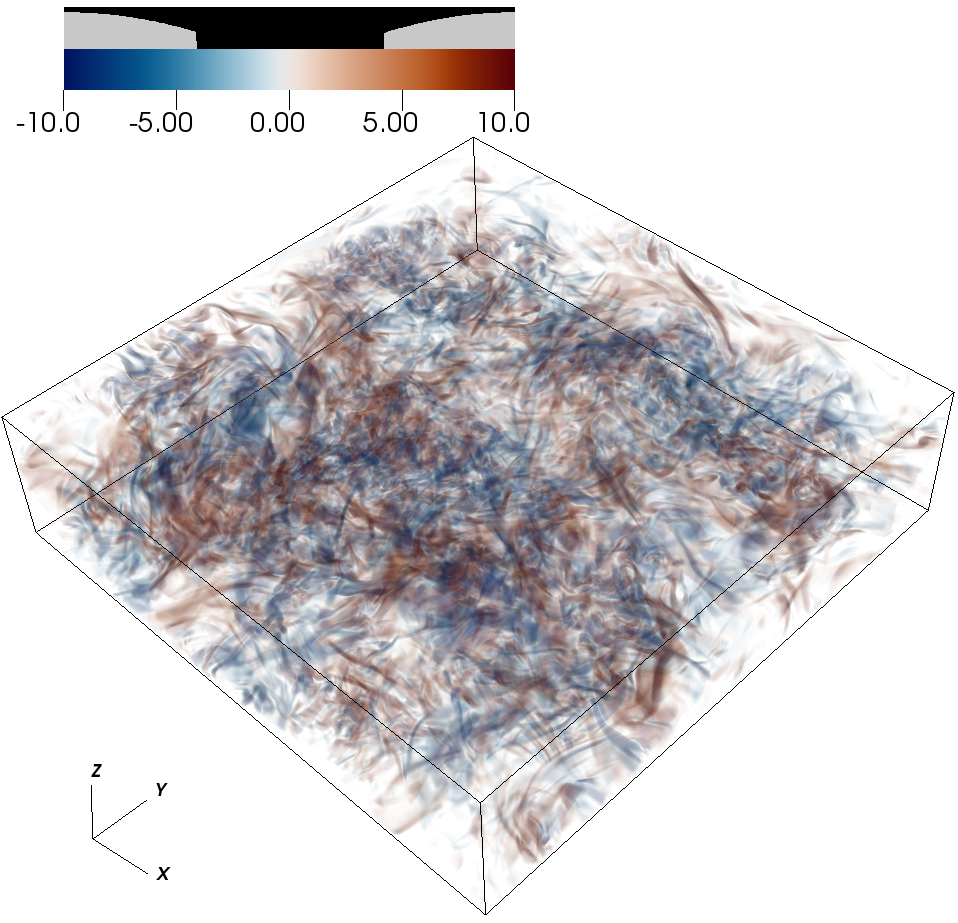
\includegraphics[width=.85\linewidth]{images/vortz_Om0.5_vr2.png}
    \emp
    \bmp{.3}
        \centering
        {\Large $Ro = .5$}

        \vspace{10pt}
        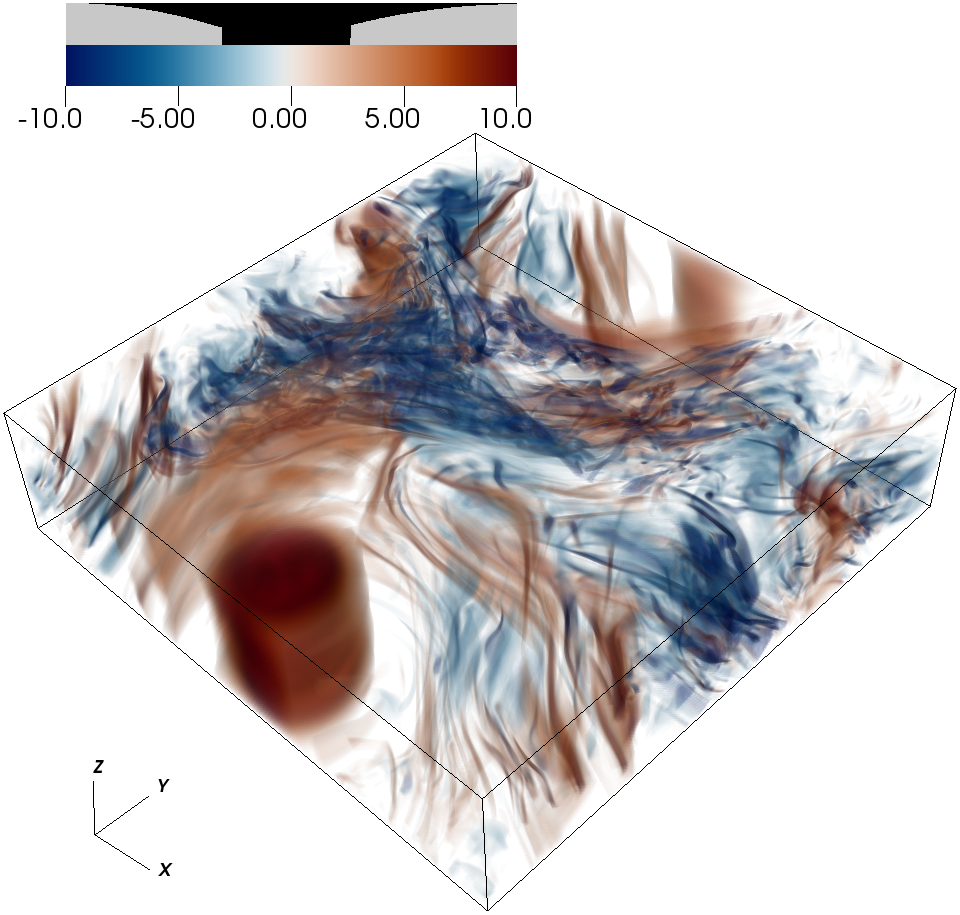
\includegraphics[width=.85\linewidth]{images/vortz_Om2_vr2.png}
    \emp
    \bmp{.3}
        \centering
        {\Large $Ro = .1$}

        \vspace{10pt}
        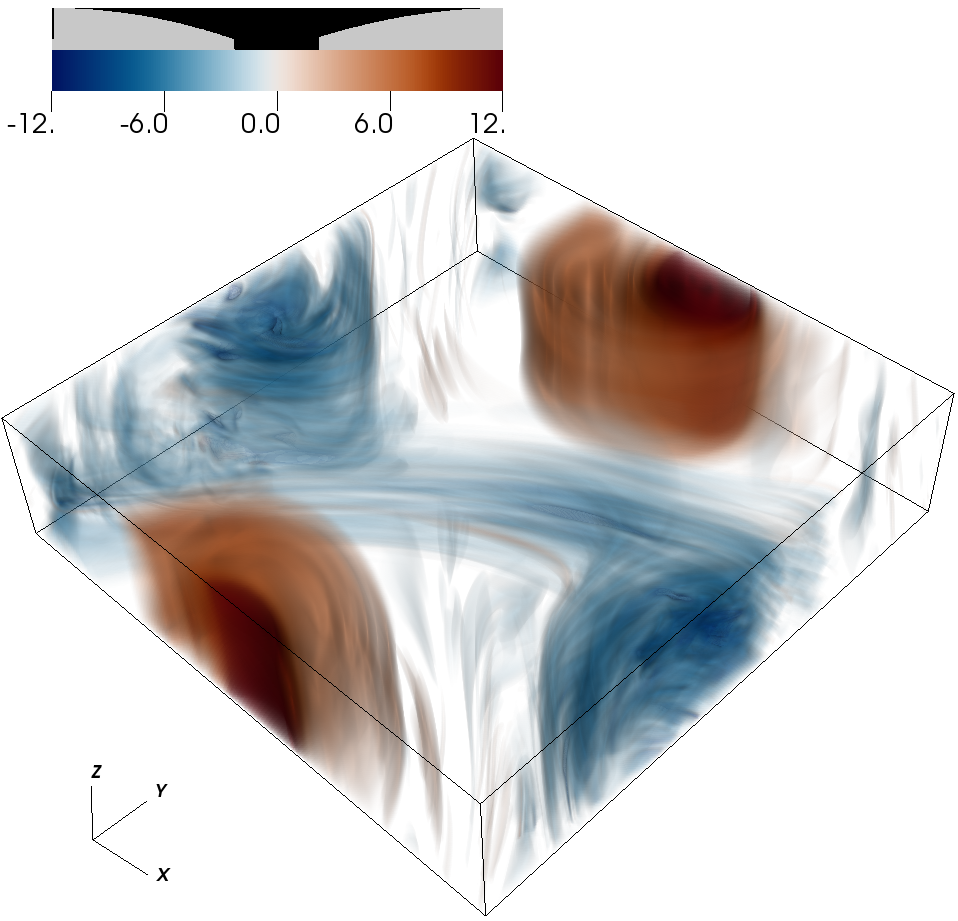
\includegraphics[width=.85\linewidth]{images/vortz_Om10_vr2.png}
    \emp

    \bmp{.09}
        \centering
        {\Large $|\nabla T|^2$}
    \emp
    \bmp{.30}
        \centering
        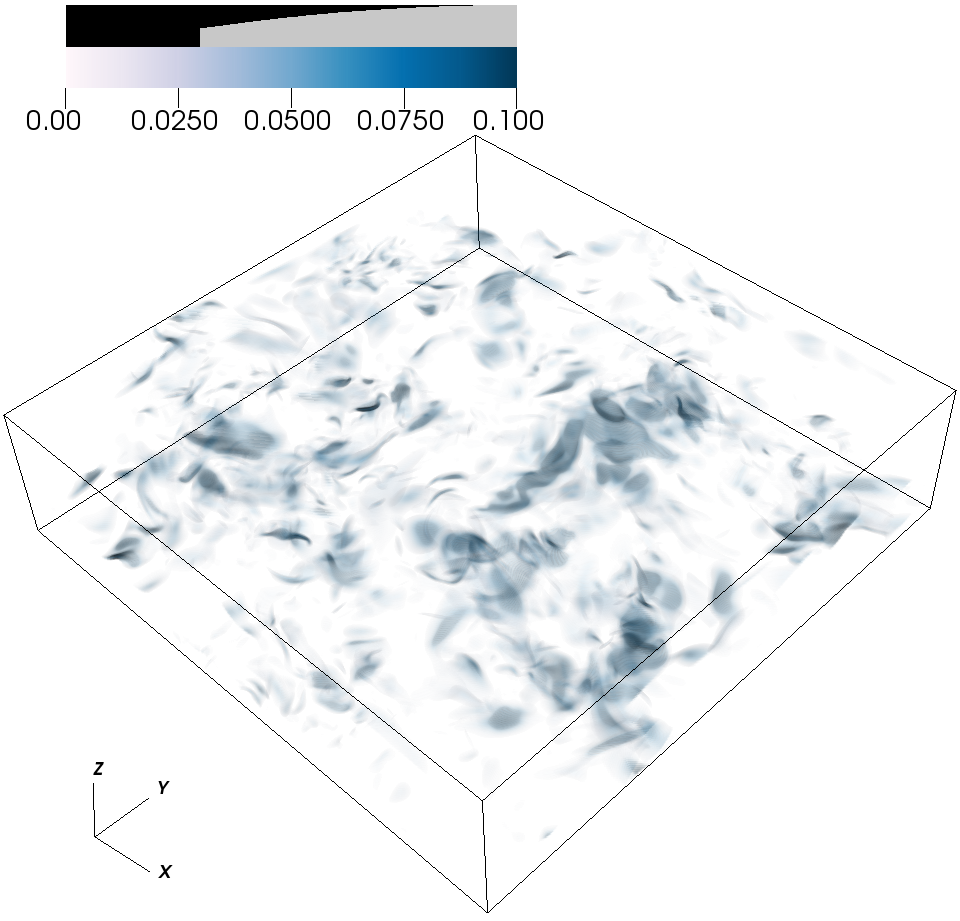
\includegraphics[width=.85\linewidth]{images/chi_Om0.5_vr2.png}
    \emp
    \bmp{.30}
        \centering
        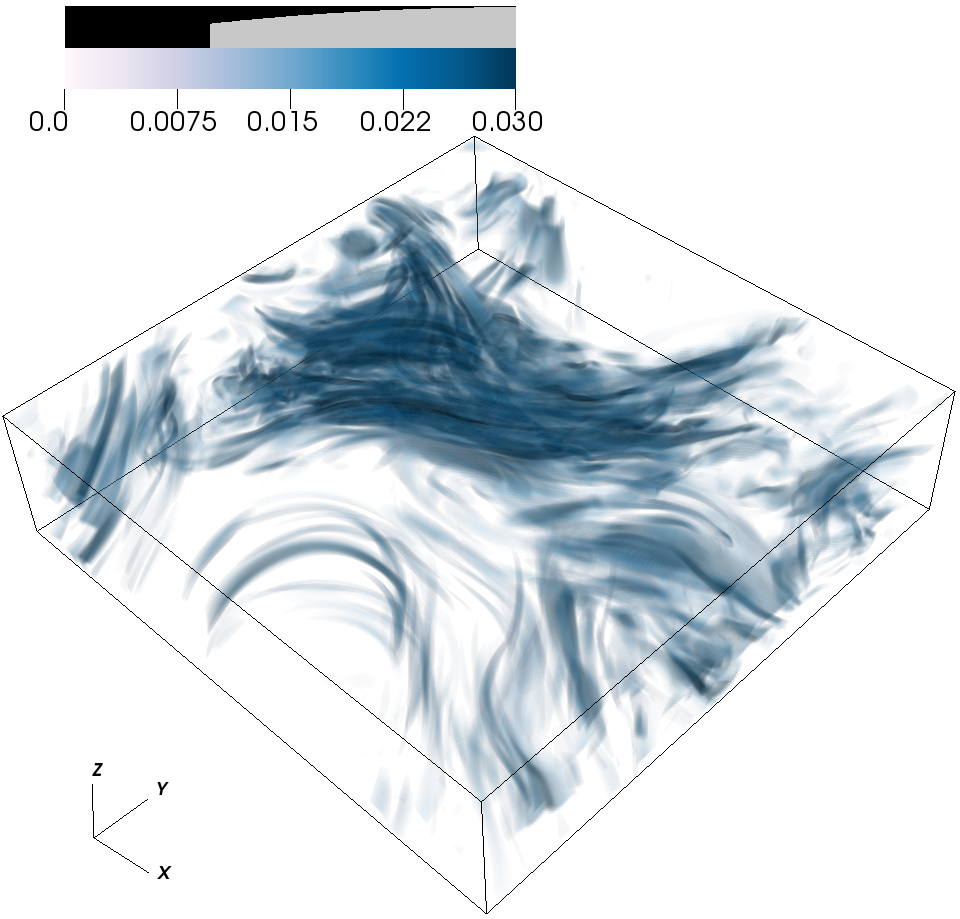
\includegraphics[width=.85\linewidth]{images/chi_Om2_vr2.png}
    \emp
    \bmp{.30}
        \centering
        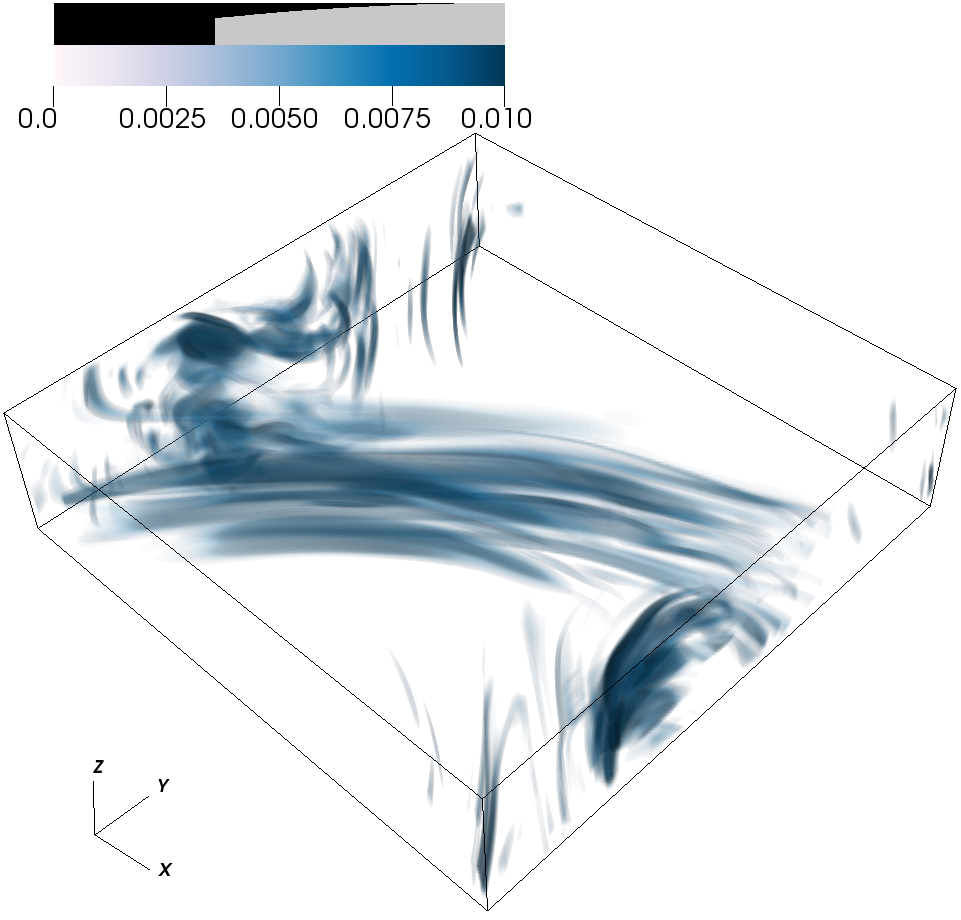
\includegraphics[width=.85\linewidth]{images/chi_Om10_vr2.png}
    \emp

    \bmp{0.09}
        \centering
        {\Large Energy Spectra}
    \emp
    \bmp{.3}
        \centering
        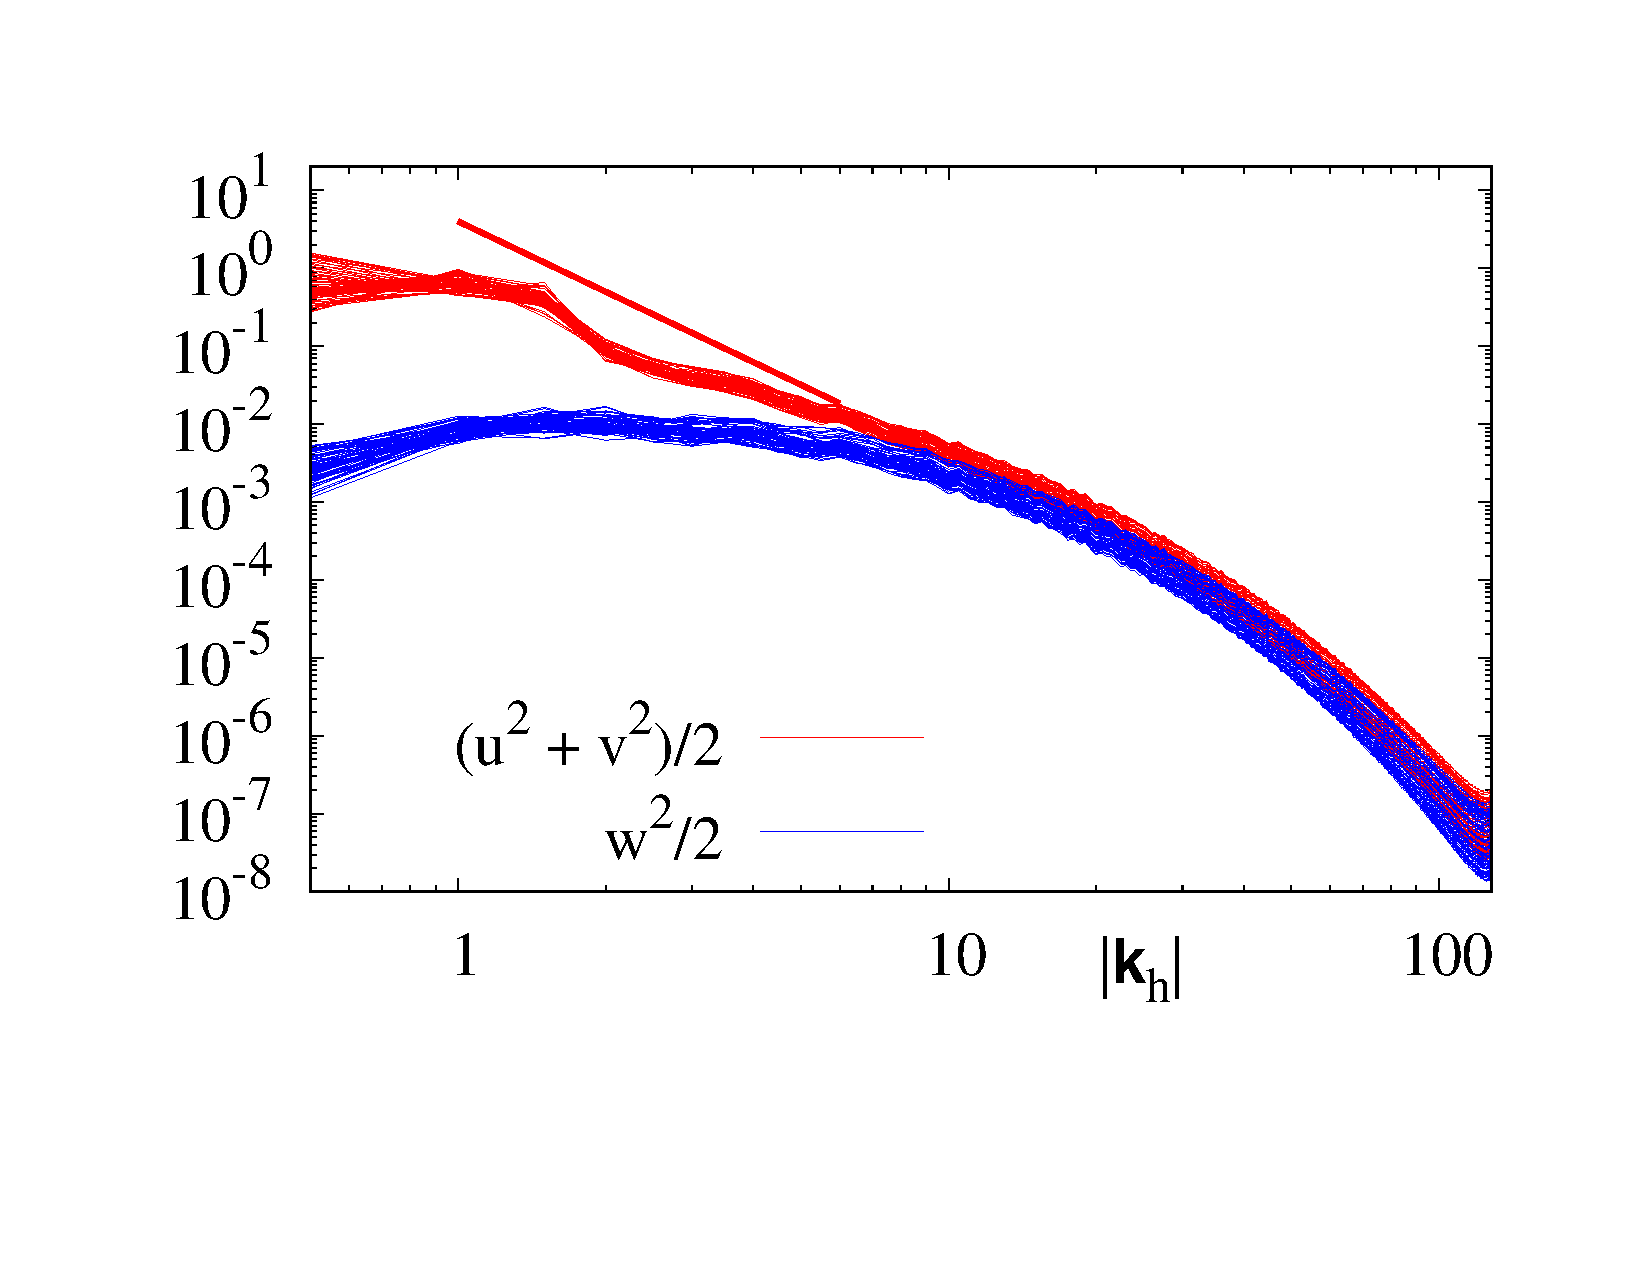
\includegraphics[width=.9\linewidth]{images/Om0.5Spec.pdf}
    \emp
    \bmp{.3}
        \centering
        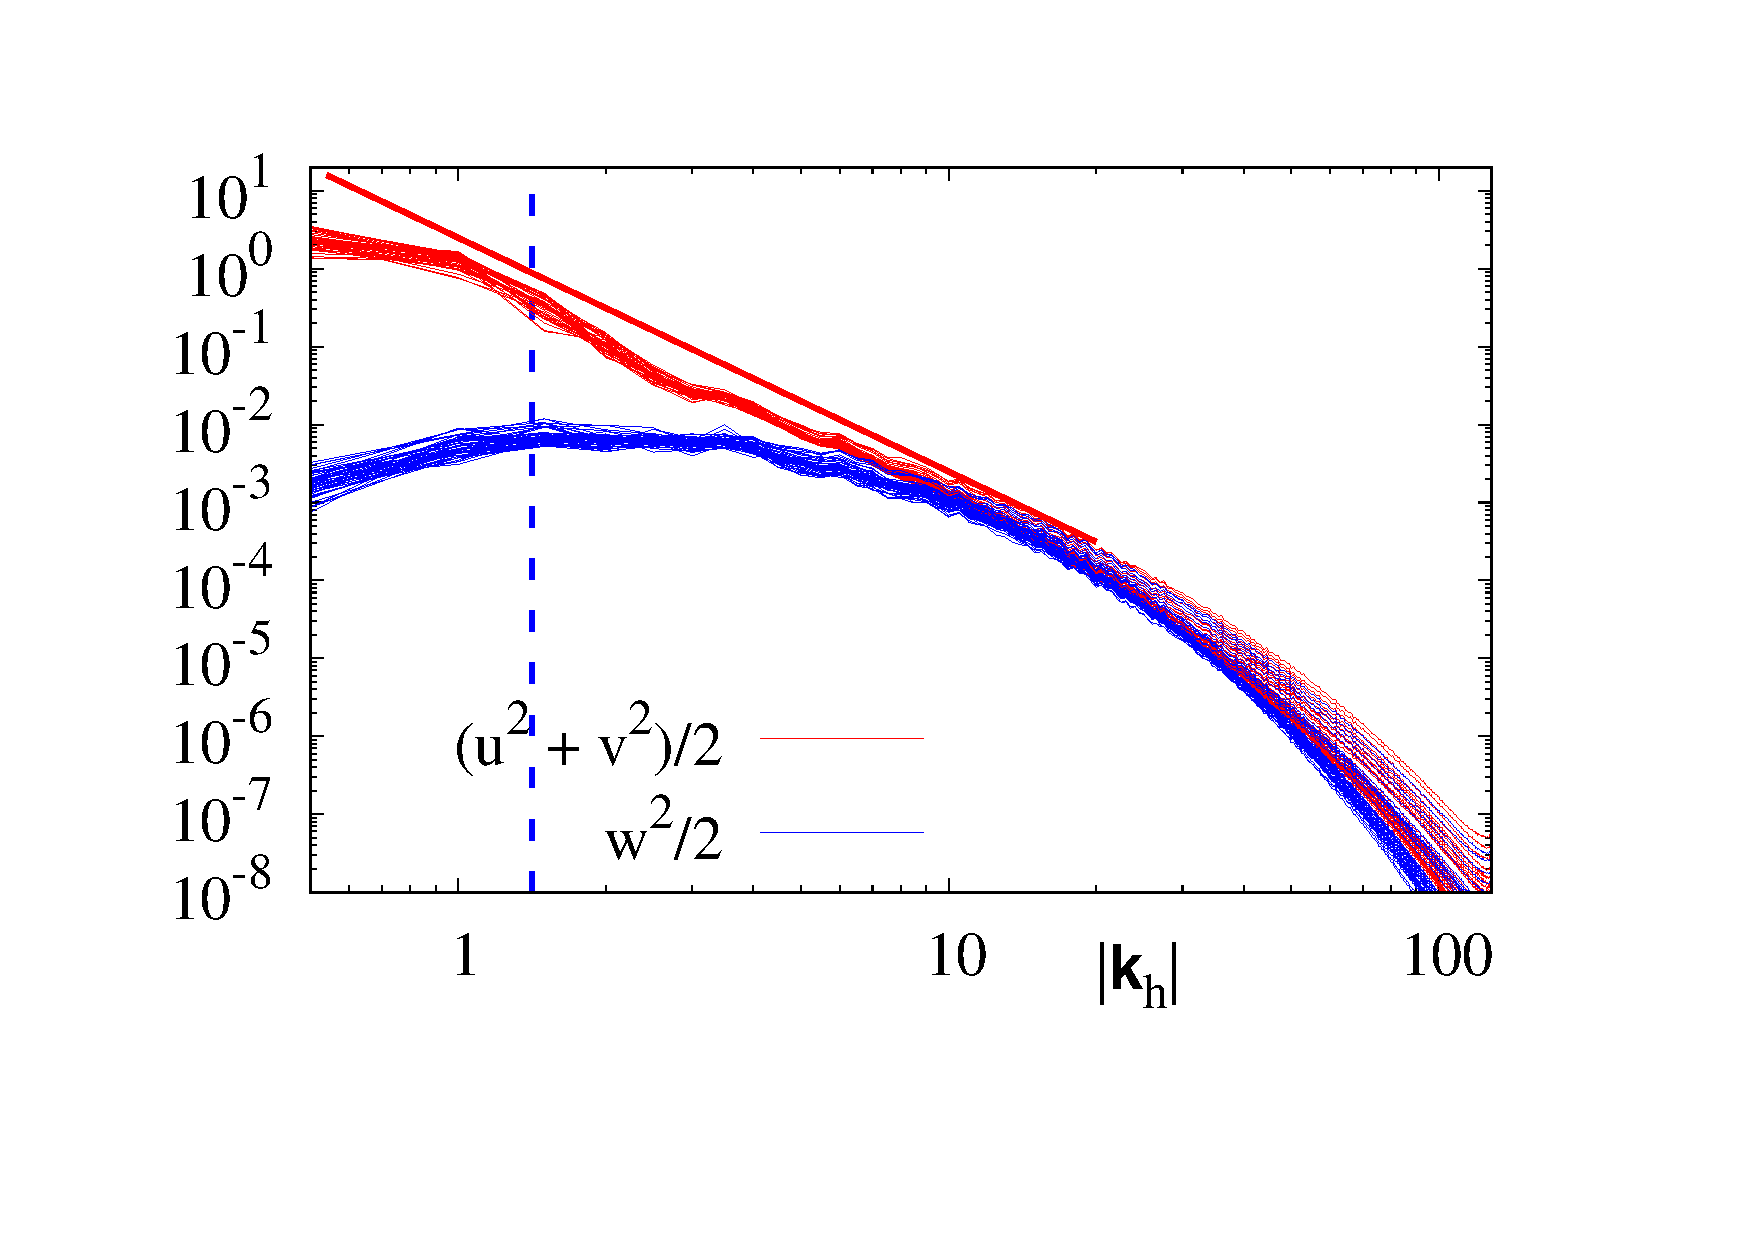
\includegraphics[width=.9\linewidth]{images/Om2Spec.pdf}
    \emp
    \bmp{.3}
        \centering
        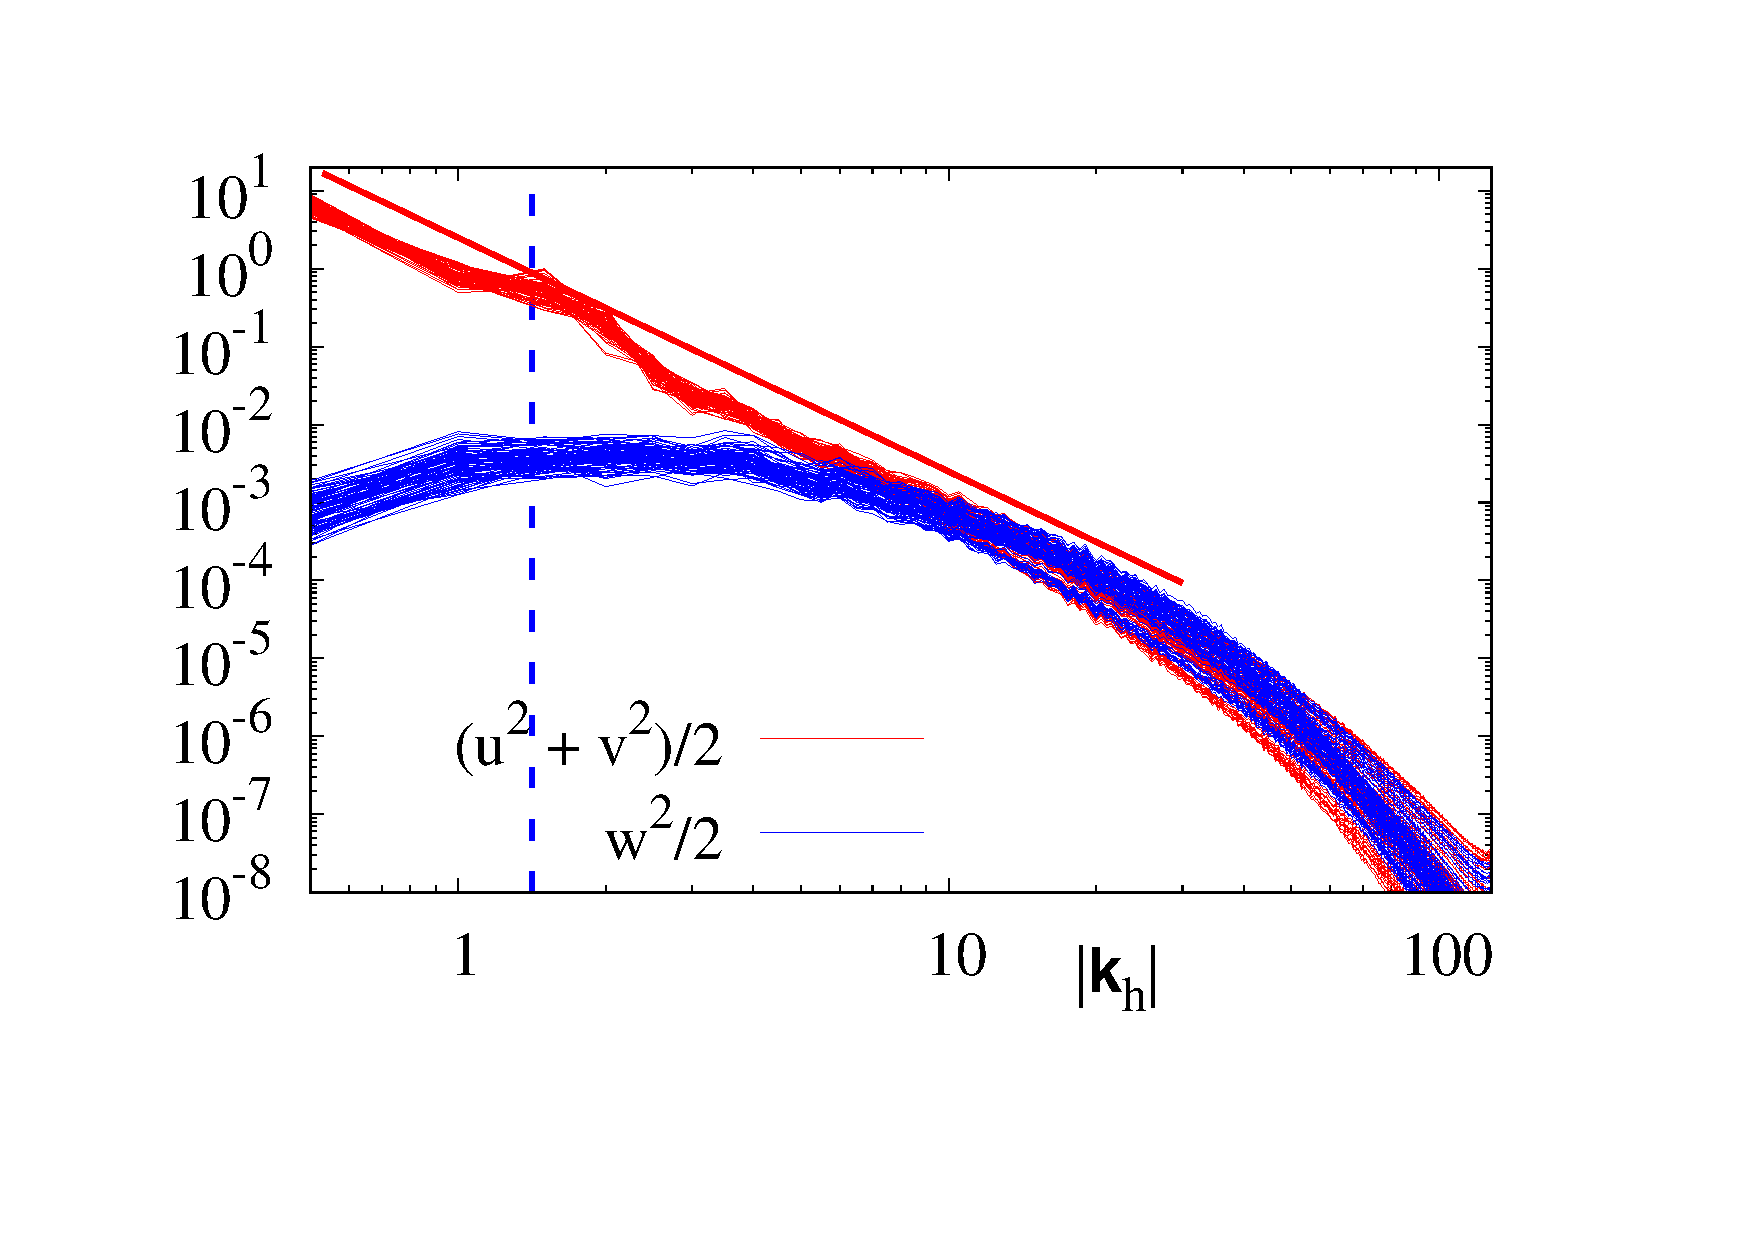
\includegraphics[width=.9\linewidth]{images/Om5Spec.pdf}
    \emp
    \end{center}
}

\block{RMS Data}{
    \centering

    \bmp{.3}
    From simulations which have reached a statistically stationary state
    (filled circles) we extract time and volume averages of quantities of
    interest (open circles have not reached a statistically stationary state
    yet, but are shown for comparison).
    \begin{gather*}
        |\uvec_h|_{\text{rms}} = \langle u^2 + v^2\rangle^{1/2}\\
        \chi = \left<|\grad T|^2\right>\\
        \eta = \frac{\chi/(PeFr^2)}{\chi/(PeFr^2) + \left<|\grad \uvec|^2\right>/Re}
    \end{gather*}
    They are shown on the right as a function of the inverse Rossby number for
    both moderate and strong stratification. The horizontal velocities increase
    proportionally to the rotation rate owing to the inverse cascade. For very
    large rotation rates, we see a decrease in the rms vertical velocity as well
    as the temperature dissipation $\chi$ associated with the increasing volume
    fraction of the domain occupied by the vortices. 

    %can observe adjustments to the rms horizontal and
    %vertical velocities (top left and right) and to the rms temperature
    %flux and mixing efficiency (bottom left and right) as the inverse Rossby number
    %varies. Each of these quantities react differently to the
    %changes by the Rossby number, however, most prominent is the increase in the
    %average horizontal velocity and appears to scale by twice the inverse Rossby
    %number. The vertical velocity in the nonrotating case should scale by the
    %Froude number (Chini {\em et al} 2022, Shah {\em et al} 2024). This scale separation between
    %simulation sets becomes less distinct as the inverse Rossby number
    %increases. Adjustments to the temperature flux and mixing efficiency are
    %less much less prominent, and the effect of rotation on these quantities is
    %unclear from these plots.

    \emp
    \bmp{.7}
        \centering
        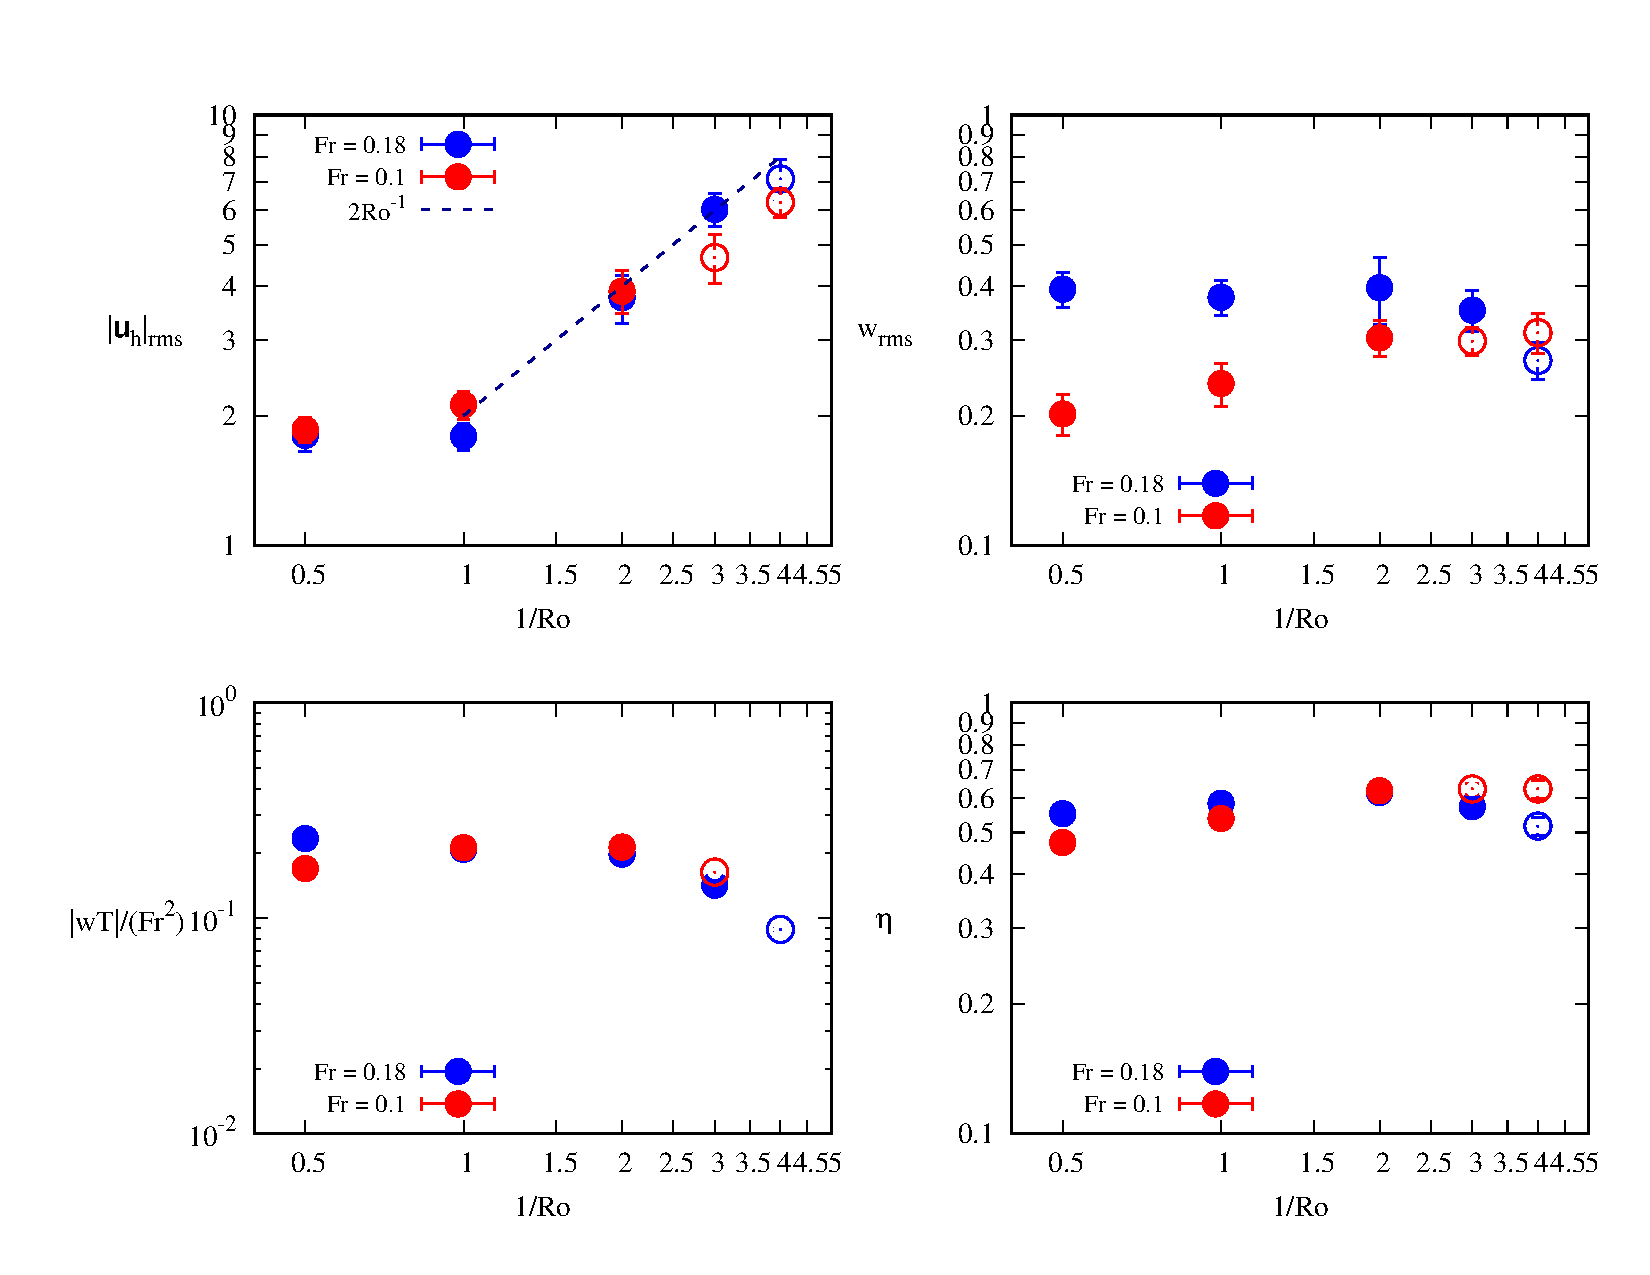
\includegraphics[width=\linewidth]{images/subplots.pdf}
    \emp
}


%%%%%%%%%%%%%%%%%%%%%%%%%%%%%%%%%%%%%%%%%%%%%%%%%%%%%%%%
\column{0.33}
%%%%%%%%%%%%%%%%%%%%%%%%%%%%%%%%%%%%%%%%%%%%%%%%%%%%%%%%

\block{Vertically Averaged Quantities}{


    We aim to characterize the properties of the vortices. We define an
    effective Rossby number,
    \begin{gather*}
        Ro_{\text{eff}}^{-1} = |\widehat{\omega}_z + Ro^{-1}|, \quad
        \text{ where } \widehat{(\cdot)} = \frac{1}{L_z}\int (\cdot) dz
    \end{gather*}
    The following figures compare 2D maps of $Ro_{\text{eff}}^{-1}$,
    $\widehat{w^2}^{1/2}$, $\widehat{|\grad T|^2}$, $\widehat{wT}$ for 4 different
    simulations at moderate and strong stratification and moderate and strong
    rotation. We see that when $Ro_{text{eff}}^{-1}$ exceeds a critical
    threshold, which appears to depend on the Froude number,  
    thermal dissipation and vertical velocity are suppressed. 
    %This method of correlation is heavily dependent on the colorbar used to
    %measure the local rotation rate. Using $2\sqrt{Fr^{-1}}$ as the center of
    %a divergent colormap appears to demonstrate a strong correlation between the
    %regions of rapid cyclonic rotation and regions of little thermal mixing and
    %vertical flow. Further investigation into the criterion for vertical mixing
    %and flow in the domain is necessary to better understand exactly how the
    %barotropic structures inhibit mixing and vertical motion within the flow. 

    \begin{center}
    \bmp{.5}
        \centering
        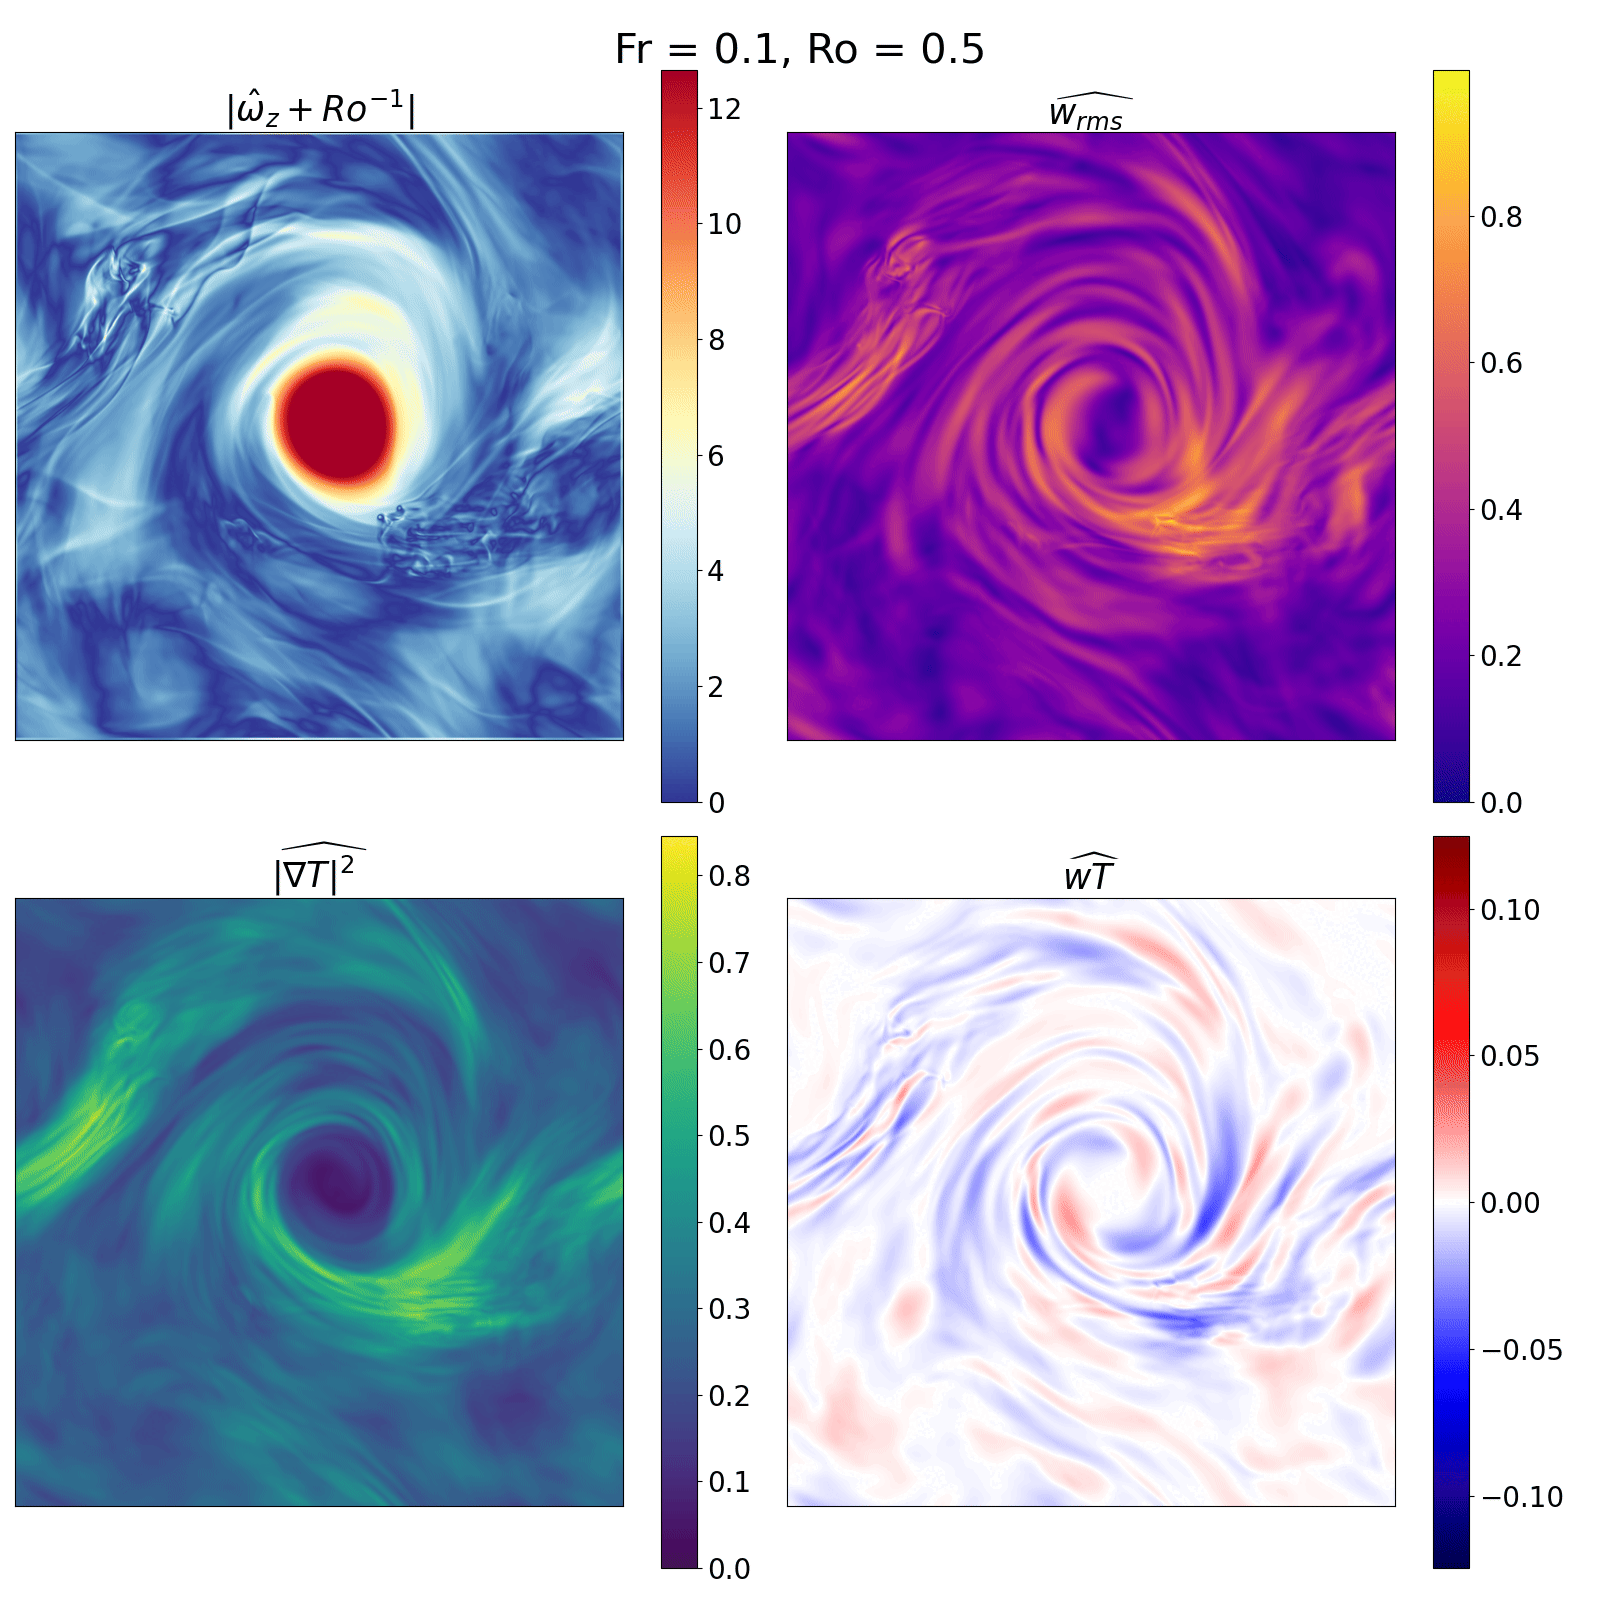
\includegraphics[width=.95\linewidth]{images/Om2B100Re600Pe60_vert_avg.png}
    \emp
    \bmp{.5}
        \centering
        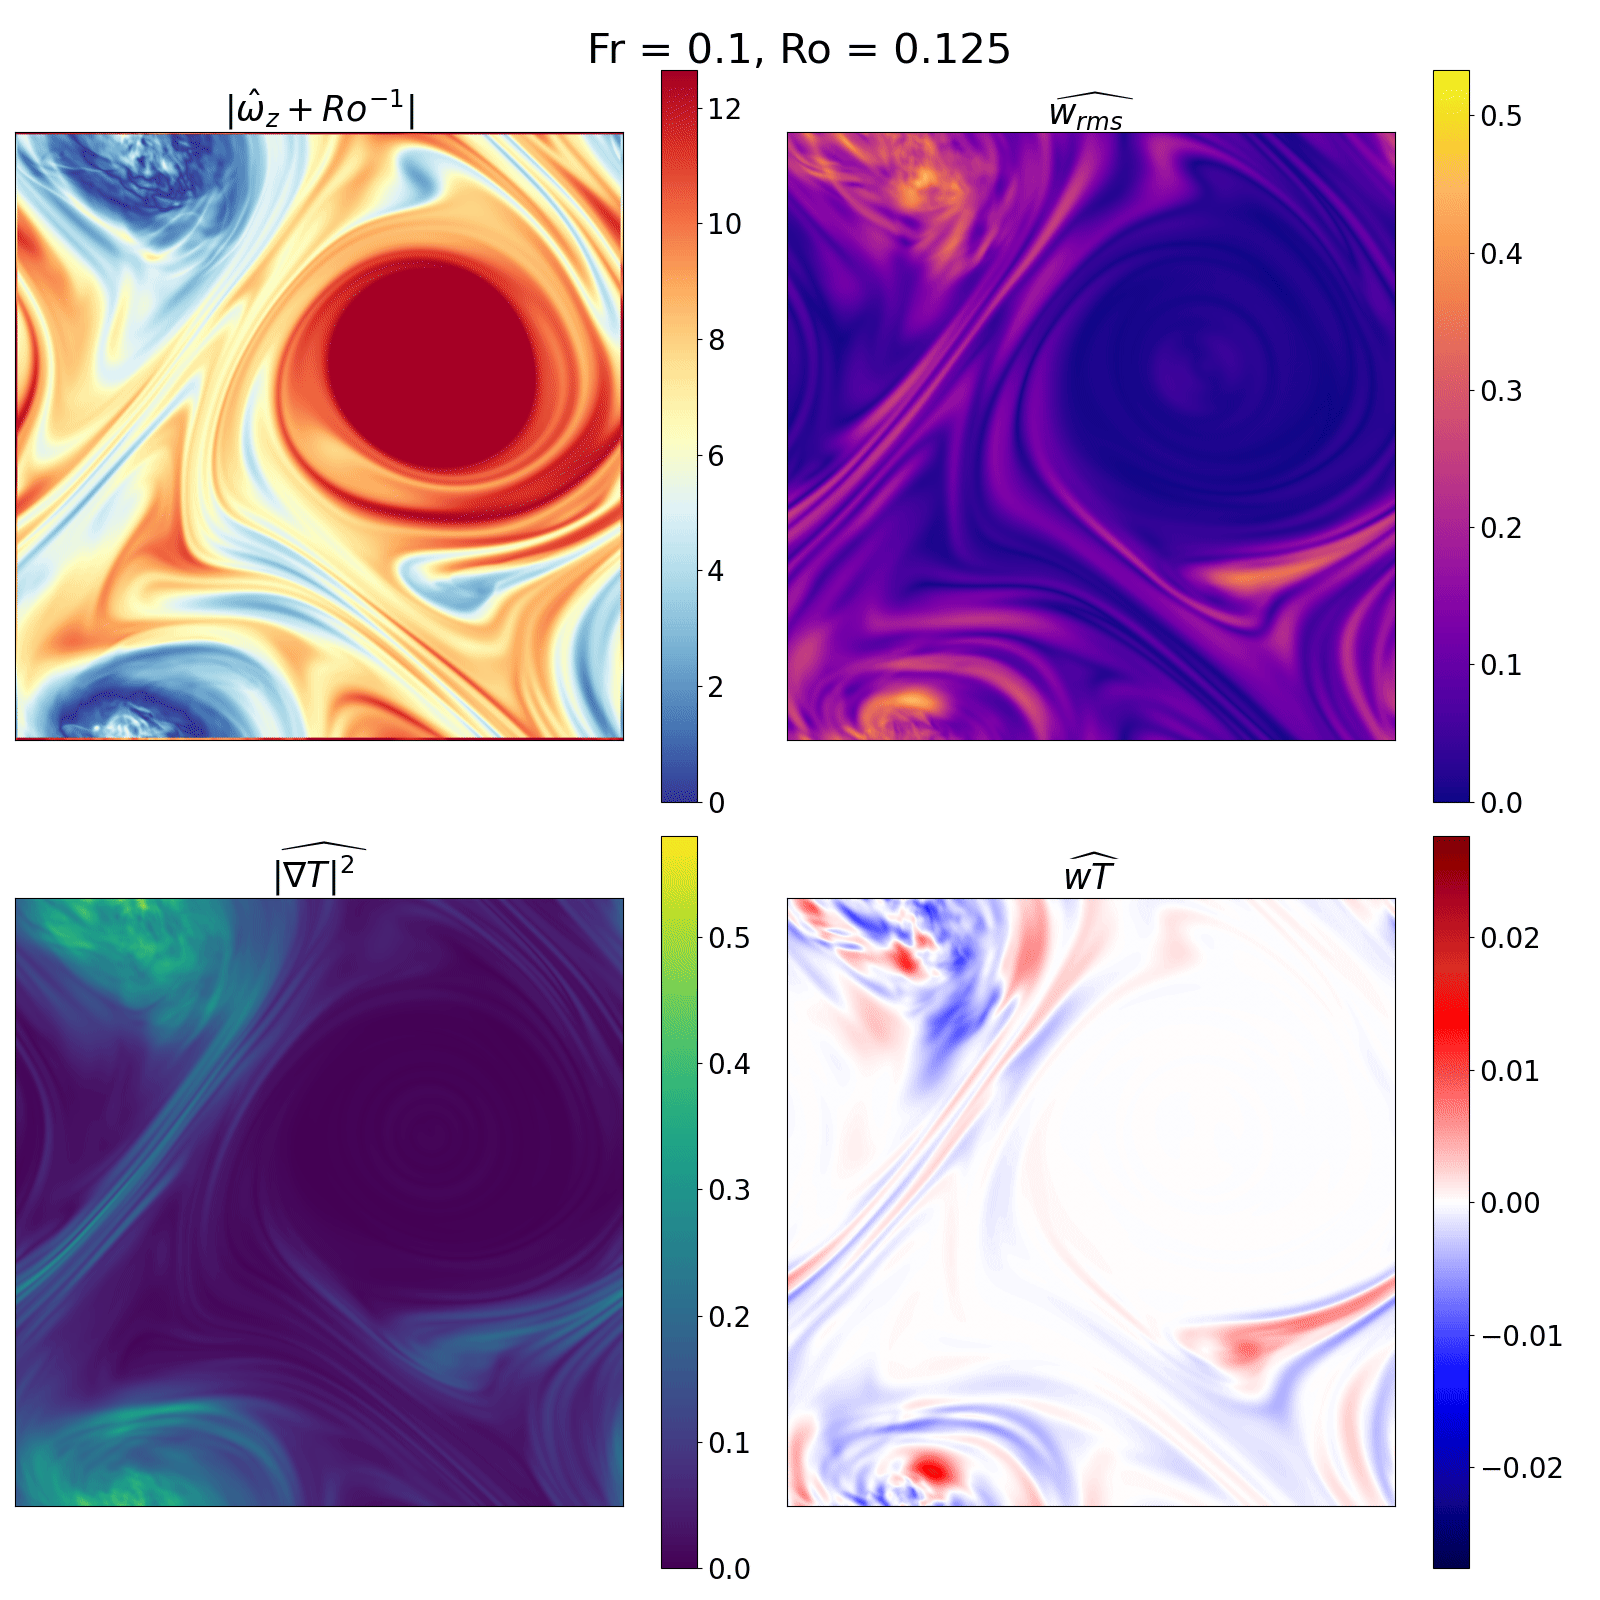
\includegraphics[width=.95\linewidth]{images/Om8B100Re600Pe60_vert_avg.png}
    \emp

    \bmp{.5}
        \centering
        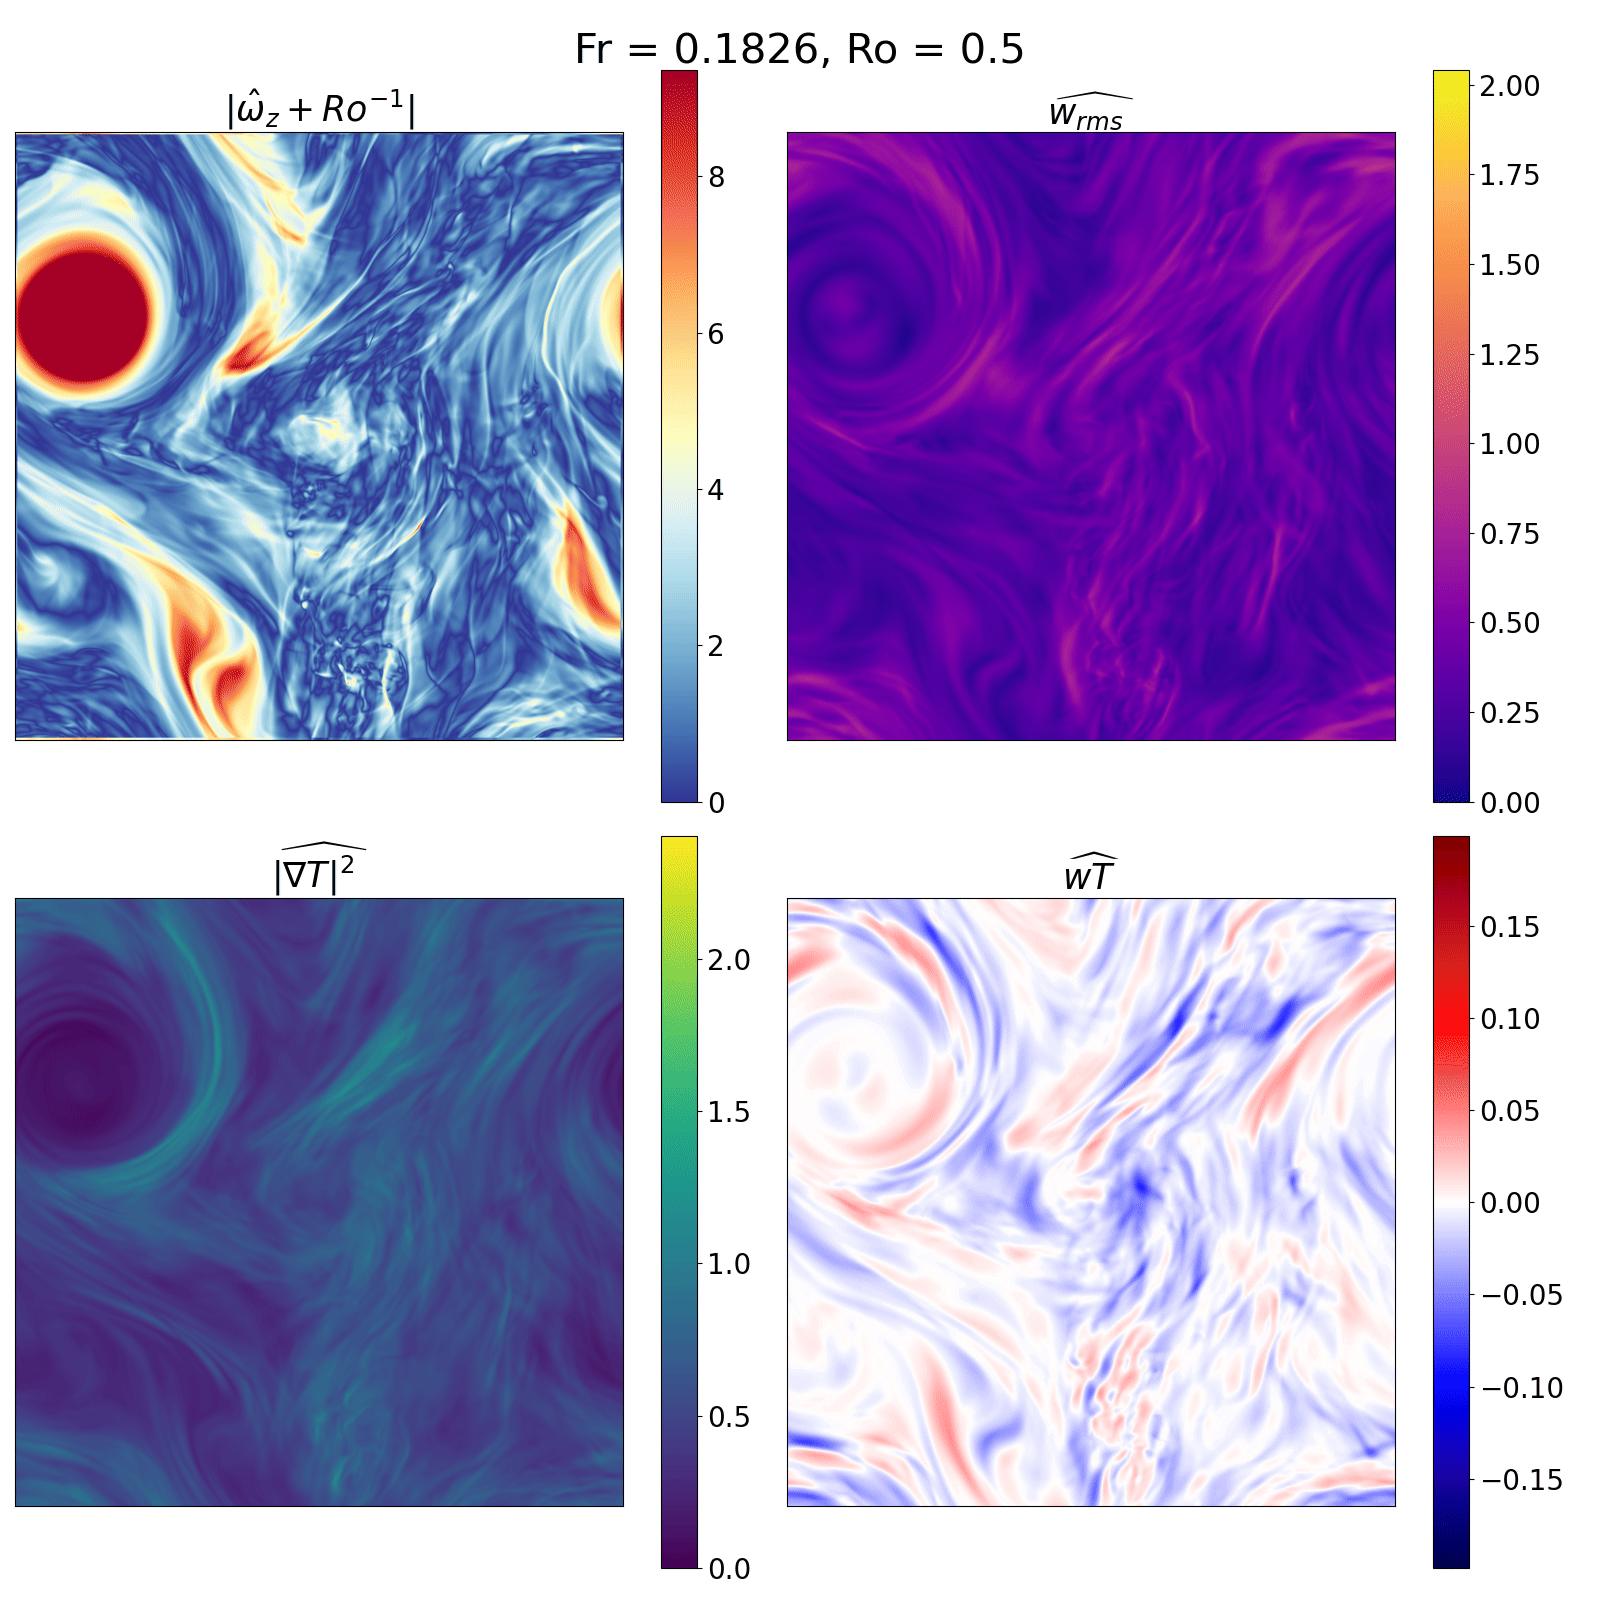
\includegraphics[width=.95\linewidth]{images/Om2B30Re600Pe60_vert_avg.png}
    \emp
    \bmp{.5}
        \centering
        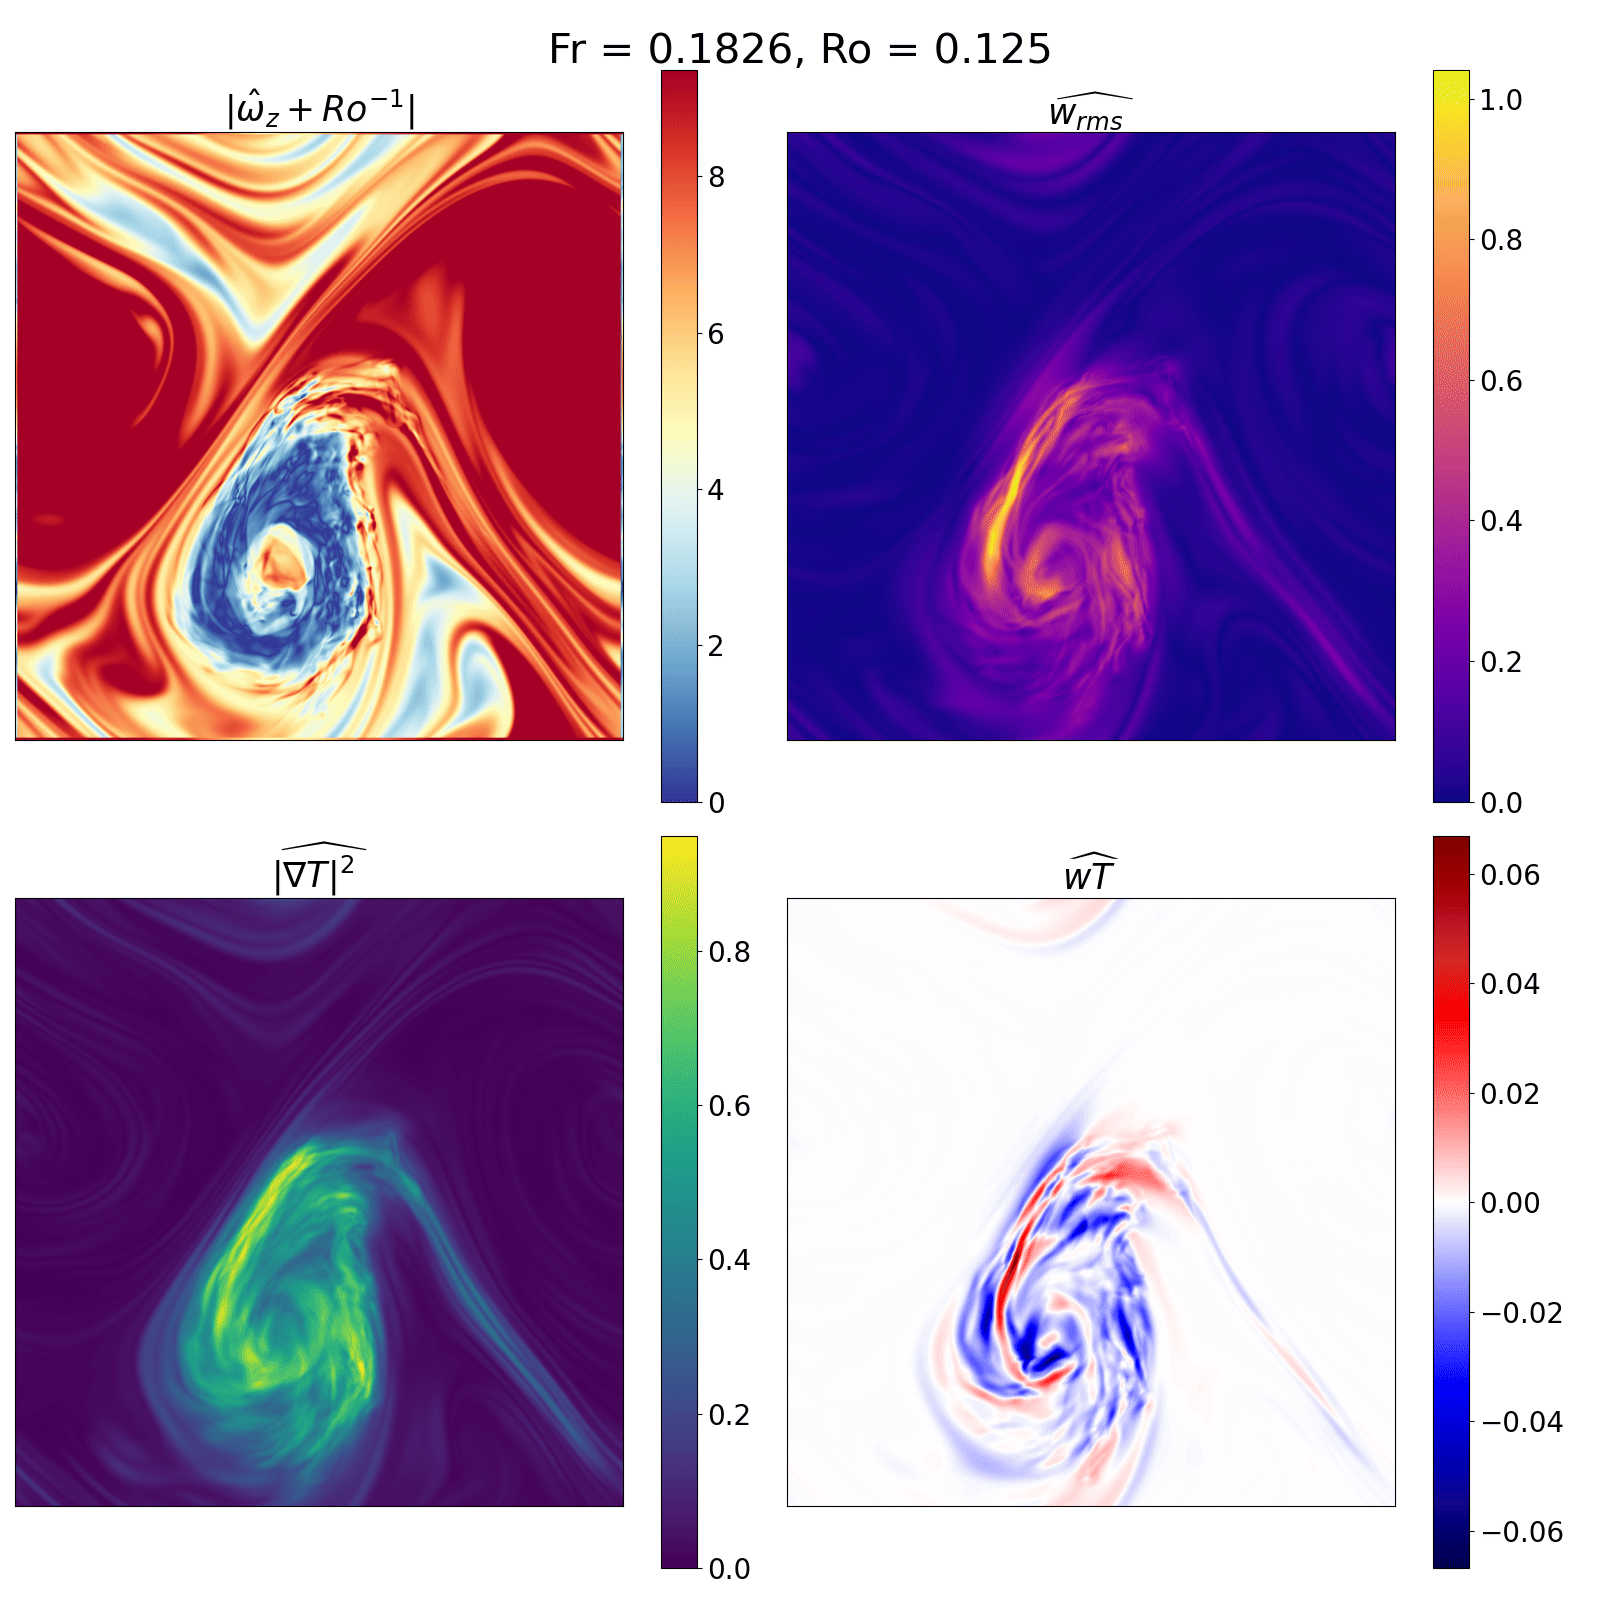
\includegraphics[width=.95\linewidth]{images/Om8B30Re600Pe60_vert_avg.png}
    \emp
    \end{center}
}


\block{References \& Acknowledgements}{
This work is supported by NSF AST-2408025. 
\\

\textbf{References}\\
Gregory P. Chini, Guillaume Michel, Keith Julien, Cesar B. Rocha, and Colm-
cille P. Caulfield. Exploiting self-organized criticality in strongly stratified
turbulence. Journal of Fluid Mechanics, 933:A22, February 2022. doi:
10.1017/jfm.2021.1060.
\\

Kasturi Shah, Gregory P. Chini, Colm-cille P. Caulfield, and Pascale Garaud.
Regimes of stratified turbulence at low Prandtl number. arXiv e-prints, art.
arXiv:2311.06424, November 2023.
\\

Michael L. Waite and Peter Bartello. Stratified turbulence dominated by
vertical motion. Journal of Fluid Mechanics, 517:281–308, 2004. doi:
10.1017/S0022112004000977.

}

\end{columns}


\end{document}
